% Options for packages loaded elsewhere
\PassOptionsToPackage{unicode}{hyperref}
\PassOptionsToPackage{hyphens}{url}
%
\documentclass[
]{book}
\usepackage{amsmath,amssymb}
\usepackage{lmodern}
\usepackage{iftex}
\ifPDFTeX
  \usepackage[T1]{fontenc}
  \usepackage[utf8]{inputenc}
  \usepackage{textcomp} % provide euro and other symbols
\else % if luatex or xetex
  \usepackage{unicode-math}
  \defaultfontfeatures{Scale=MatchLowercase}
  \defaultfontfeatures[\rmfamily]{Ligatures=TeX,Scale=1}
\fi
% Use upquote if available, for straight quotes in verbatim environments
\IfFileExists{upquote.sty}{\usepackage{upquote}}{}
\IfFileExists{microtype.sty}{% use microtype if available
  \usepackage[]{microtype}
  \UseMicrotypeSet[protrusion]{basicmath} % disable protrusion for tt fonts
}{}
\makeatletter
\@ifundefined{KOMAClassName}{% if non-KOMA class
  \IfFileExists{parskip.sty}{%
    \usepackage{parskip}
  }{% else
    \setlength{\parindent}{0pt}
    \setlength{\parskip}{6pt plus 2pt minus 1pt}}
}{% if KOMA class
  \KOMAoptions{parskip=half}}
\makeatother
\usepackage{xcolor}
\IfFileExists{xurl.sty}{\usepackage{xurl}}{} % add URL line breaks if available
\IfFileExists{bookmark.sty}{\usepackage{bookmark}}{\usepackage{hyperref}}
\hypersetup{
  pdftitle={Intro Data Science long project},
  pdfauthor={Pedro Miguel de Sousa Magalhães},
  hidelinks,
  pdfcreator={LaTeX via pandoc}}
\urlstyle{same} % disable monospaced font for URLs
\usepackage{color}
\usepackage{fancyvrb}
\newcommand{\VerbBar}{|}
\newcommand{\VERB}{\Verb[commandchars=\\\{\}]}
\DefineVerbatimEnvironment{Highlighting}{Verbatim}{commandchars=\\\{\}}
% Add ',fontsize=\small' for more characters per line
\usepackage{framed}
\definecolor{shadecolor}{RGB}{248,248,248}
\newenvironment{Shaded}{\begin{snugshade}}{\end{snugshade}}
\newcommand{\AlertTok}[1]{\textcolor[rgb]{0.94,0.16,0.16}{#1}}
\newcommand{\AnnotationTok}[1]{\textcolor[rgb]{0.56,0.35,0.01}{\textbf{\textit{#1}}}}
\newcommand{\AttributeTok}[1]{\textcolor[rgb]{0.77,0.63,0.00}{#1}}
\newcommand{\BaseNTok}[1]{\textcolor[rgb]{0.00,0.00,0.81}{#1}}
\newcommand{\BuiltInTok}[1]{#1}
\newcommand{\CharTok}[1]{\textcolor[rgb]{0.31,0.60,0.02}{#1}}
\newcommand{\CommentTok}[1]{\textcolor[rgb]{0.56,0.35,0.01}{\textit{#1}}}
\newcommand{\CommentVarTok}[1]{\textcolor[rgb]{0.56,0.35,0.01}{\textbf{\textit{#1}}}}
\newcommand{\ConstantTok}[1]{\textcolor[rgb]{0.00,0.00,0.00}{#1}}
\newcommand{\ControlFlowTok}[1]{\textcolor[rgb]{0.13,0.29,0.53}{\textbf{#1}}}
\newcommand{\DataTypeTok}[1]{\textcolor[rgb]{0.13,0.29,0.53}{#1}}
\newcommand{\DecValTok}[1]{\textcolor[rgb]{0.00,0.00,0.81}{#1}}
\newcommand{\DocumentationTok}[1]{\textcolor[rgb]{0.56,0.35,0.01}{\textbf{\textit{#1}}}}
\newcommand{\ErrorTok}[1]{\textcolor[rgb]{0.64,0.00,0.00}{\textbf{#1}}}
\newcommand{\ExtensionTok}[1]{#1}
\newcommand{\FloatTok}[1]{\textcolor[rgb]{0.00,0.00,0.81}{#1}}
\newcommand{\FunctionTok}[1]{\textcolor[rgb]{0.00,0.00,0.00}{#1}}
\newcommand{\ImportTok}[1]{#1}
\newcommand{\InformationTok}[1]{\textcolor[rgb]{0.56,0.35,0.01}{\textbf{\textit{#1}}}}
\newcommand{\KeywordTok}[1]{\textcolor[rgb]{0.13,0.29,0.53}{\textbf{#1}}}
\newcommand{\NormalTok}[1]{#1}
\newcommand{\OperatorTok}[1]{\textcolor[rgb]{0.81,0.36,0.00}{\textbf{#1}}}
\newcommand{\OtherTok}[1]{\textcolor[rgb]{0.56,0.35,0.01}{#1}}
\newcommand{\PreprocessorTok}[1]{\textcolor[rgb]{0.56,0.35,0.01}{\textit{#1}}}
\newcommand{\RegionMarkerTok}[1]{#1}
\newcommand{\SpecialCharTok}[1]{\textcolor[rgb]{0.00,0.00,0.00}{#1}}
\newcommand{\SpecialStringTok}[1]{\textcolor[rgb]{0.31,0.60,0.02}{#1}}
\newcommand{\StringTok}[1]{\textcolor[rgb]{0.31,0.60,0.02}{#1}}
\newcommand{\VariableTok}[1]{\textcolor[rgb]{0.00,0.00,0.00}{#1}}
\newcommand{\VerbatimStringTok}[1]{\textcolor[rgb]{0.31,0.60,0.02}{#1}}
\newcommand{\WarningTok}[1]{\textcolor[rgb]{0.56,0.35,0.01}{\textbf{\textit{#1}}}}
\usepackage{longtable,booktabs,array}
\usepackage{calc} % for calculating minipage widths
% Correct order of tables after \paragraph or \subparagraph
\usepackage{etoolbox}
\makeatletter
\patchcmd\longtable{\par}{\if@noskipsec\mbox{}\fi\par}{}{}
\makeatother
% Allow footnotes in longtable head/foot
\IfFileExists{footnotehyper.sty}{\usepackage{footnotehyper}}{\usepackage{footnote}}
\makesavenoteenv{longtable}
\usepackage{graphicx}
\makeatletter
\def\maxwidth{\ifdim\Gin@nat@width>\linewidth\linewidth\else\Gin@nat@width\fi}
\def\maxheight{\ifdim\Gin@nat@height>\textheight\textheight\else\Gin@nat@height\fi}
\makeatother
% Scale images if necessary, so that they will not overflow the page
% margins by default, and it is still possible to overwrite the defaults
% using explicit options in \includegraphics[width, height, ...]{}
\setkeys{Gin}{width=\maxwidth,height=\maxheight,keepaspectratio}
% Set default figure placement to htbp
\makeatletter
\def\fps@figure{htbp}
\makeatother
\setlength{\emergencystretch}{3em} % prevent overfull lines
\providecommand{\tightlist}{%
  \setlength{\itemsep}{0pt}\setlength{\parskip}{0pt}}
\setcounter{secnumdepth}{5}
\usepackage{booktabs}
\ifLuaTeX
  \usepackage{selnolig}  % disable illegal ligatures
\fi
\usepackage[]{natbib}
\bibliographystyle{plainnat}

\title{Intro Data Science long project}
\author{Pedro Miguel de Sousa Magalhães}
\date{2022-01-14}

\begin{document}
\maketitle

{
\setcounter{tocdepth}{1}
\tableofcontents
}
\hypertarget{introduction}{%
\chapter{Introduction}\label{introduction}}

\hypertarget{students-commitment}{%
\section{Students commitment}\label{students-commitment}}

\begin{quote}
Declaro que o presente relatório é de minha autoria e não foi utilizado previamente noutro curso ou unidade curricular, desta ou de outra instituição. As referências a outros autores (afirmações,ideias, pensamentos) respeitam escrupulosamente as regras da atribuição, e encontramse devidamente indicadas no texto e nas referências bibliográficas, de acordo com as normas dereferenciação. Tenho consciência de que a prática de plágio e auto-plágio constitui um ilícito académico.
\end{quote}

\hypertarget{software-information}{%
\section{Software information}\label{software-information}}

The R session information when building this project is has shown below:

\begin{Shaded}
\begin{Highlighting}[]
\FunctionTok{sessionInfo}\NormalTok{()}
\end{Highlighting}
\end{Shaded}

\begin{verbatim}
## R version 3.5.3 (2019-03-11)
## Platform: x86_64-w64-mingw32/x64 (64-bit)
## Running under: Windows 10 x64 (build 19042)
## 
## Matrix products: default
## 
## locale:
## [1] LC_COLLATE=Portuguese_Portugal.1252  LC_CTYPE=Portuguese_Portugal.1252   
## [3] LC_MONETARY=Portuguese_Portugal.1252 LC_NUMERIC=C                        
## [5] LC_TIME=Portuguese_Portugal.1252    
## 
## attached base packages:
## [1] stats     graphics  grDevices datasets  utils     methods   base     
## 
## loaded via a namespace (and not attached):
##  [1] compiler_3.5.3  magrittr_2.0.1  bookdown_0.24   fastmap_1.1.0  
##  [5] htmltools_0.5.2 tools_3.5.3     rstudioapi_0.13 yaml_2.2.1     
##  [9] stringi_1.7.6   rmarkdown_2.11  knitr_1.37      stringr_1.4.0  
## [13] xfun_0.29       digest_0.6.29   rlang_0.4.12    renv_0.15.0    
## [17] evaluate_0.14
\end{verbatim}

\hypertarget{business-understanding}{%
\chapter{Business Understanding}\label{business-understanding}}

\hypertarget{business-objectives}{%
\section{Business objectives}\label{business-objectives}}

The client is a e-commerce company operating on the high end market. Its only known sales channel is online. They wish to improve their customers experience, and their conversion, by using the information they actively collect from each touchpoint.

Main business goal: improve conversion
How to achieve goal: understand which factors influence conversion so marketing strategy can be improved

\hypertarget{assess-situation}{%
\section{Assess Situation}\label{assess-situation}}

A Sample of customer sessions for given period of time is provided.
There is no information regarding how session was defined.
No information regarding user identification was provided and there for is not possible to use user as a perspective on the analysis or any information regarding acquisition journey. Therefore the project will focus solely on sessions, nonetheless it is important to point out the fact that a user can have several sessions which lead into a conversion and that can impact conversion strategies.

No special hardware and environment needs was identified

\hypertarget{data-mining-goals}{%
\section{Data Mining Goals}\label{data-mining-goals}}

Based on the Business Goals and the nature of the data available we can conclude this is a \textbf{binary classification problem with a focus on inference.} Therefore the following assumptions can be made about the expected output:

\begin{itemize}
\tightlist
\item
  The actual model contains valuable information to be used by the client. Therefore, black box models are less in line with the needs,
\item
  The probability of conversion is not relevant,
\item
  Each variable attribution is relevant
\end{itemize}

Throut this project we will address the following questions:

\begin{itemize}
\tightlist
\item
  Is there a relationship between a conversion and information available related to that session ?
\item
  Which is the contribution of each of the variables to conversion?
\item
  How accurately can we estimate the effect on conversion?
\item
  Is there synergy among each session elements?
\item
  Does a model surpass a naive baseline approach of assuming the most shown class?
\item
  Does Data imbalance impact output?
\end{itemize}

\hypertarget{project-plan}{%
\section{Project Plan}\label{project-plan}}

The current project was executed with the following stages:

\begin{enumerate}
\def\labelenumi{\arabic{enumi}.}
\tightlist
\item
  Explore data Analysis
\item
  Data transformations
\item
  Data preparation for modeling
\item
  Modeling
\item
  Conclusions
\end{enumerate}

The following terms will be used during this project with the following meaning:

\textbf{User:} any unique IP which has reached the store. One individual can have more than one ip,

\textbf{Client:} a user that converted, this means, it bought from the shop,

\textbf{Touchpoints:} represents any interaction between the user and the online store of any sort,

\textbf{Session:} a period of time (normally of 30 min max) during which the user interacted with the shop. Every session starts with a touchpoint. Under some conditions depending on the website metrics collection a session can have more than one touchpoint.

\hypertarget{data-aquisition-and-understanding}{%
\chapter{Data aquisition and understanding}\label{data-aquisition-and-understanding}}

Features by:
- behavior
- journey
- segment
- device and geo

\begin{Shaded}
\begin{Highlighting}[]
\FunctionTok{library}\NormalTok{(tidyverse)}
\FunctionTok{library}\NormalTok{(corrplot)}
\FunctionTok{library}\NormalTok{(car)}
\FunctionTok{library}\NormalTok{(tidymodels)}
\FunctionTok{library}\NormalTok{(mice)}
\FunctionTok{library}\NormalTok{(forecast)}

\FunctionTok{source}\NormalTok{(}\StringTok{"scripts/eda\_functions.r"}\NormalTok{)}
\end{Highlighting}
\end{Shaded}

\begin{Shaded}
\begin{Highlighting}[]
\CommentTok{\# import data}
\NormalTok{unbalanced\_data }\OtherTok{\textless{}{-}} \FunctionTok{read\_csv}\NormalTok{(}\StringTok{"./data/train\_full.csv"}\NormalTok{) }\SpecialCharTok{\%\textgreater{}\%} \FunctionTok{select}\NormalTok{(}\SpecialCharTok{{-}}\NormalTok{...}\DecValTok{1}\NormalTok{)}
\end{Highlighting}
\end{Shaded}

\begin{verbatim}
## New names:
## * `` -> ...1
\end{verbatim}

\begin{verbatim}
## Rows: 95000 Columns: 21
\end{verbatim}

\begin{verbatim}
## -- Column specification --------------------------------------------------------
## Delimiter: ","
## chr  (9): session_id, plaform, segment, customer_type, device_group, visitor...
## dbl (12): ...1, has_listing, has_used_search, has_recommendation, has_add_to...
\end{verbatim}

\begin{verbatim}
## 
## i Use `spec()` to retrieve the full column specification for this data.
## i Specify the column types or set `show_col_types = FALSE` to quiet this message.
\end{verbatim}

\begin{Shaded}
\begin{Highlighting}[]
\NormalTok{balanced\_data }\OtherTok{\textless{}{-}} \FunctionTok{read\_csv}\NormalTok{(}\StringTok{"./data/train\_balanced.csv"}\NormalTok{) }\SpecialCharTok{\%\textgreater{}\%} \FunctionTok{select}\NormalTok{(}\SpecialCharTok{{-}}\NormalTok{...}\DecValTok{1}\NormalTok{)}
\end{Highlighting}
\end{Shaded}

\begin{verbatim}
## New names:
## * `` -> ...1
\end{verbatim}

\begin{verbatim}
## Rows: 16000 Columns: 21
\end{verbatim}

\begin{verbatim}
## -- Column specification --------------------------------------------------------
## Delimiter: ","
## chr  (9): session_id, plaform, segment, customer_type, device_group, visitor...
## dbl (12): ...1, has_listing, has_used_search, has_recommendation, has_add_to...
\end{verbatim}

\begin{verbatim}
## 
## i Use `spec()` to retrieve the full column specification for this data.
## i Specify the column types or set `show_col_types = FALSE` to quiet this message.
\end{verbatim}

\begin{Shaded}
\begin{Highlighting}[]
\CommentTok{\# convert categorical and dummy to factor variable}
\NormalTok{unbalanced\_data }\OtherTok{\textless{}{-}}\NormalTok{ unbalanced\_data }\SpecialCharTok{\%\textgreater{}\%} 
  \FunctionTok{mutate\_at}\NormalTok{(}\FunctionTok{vars}\NormalTok{(}
    \SpecialCharTok{!}\FunctionTok{contains}\NormalTok{(}\FunctionTok{c}\NormalTok{(}\StringTok{"duration"}\NormalTok{, }\StringTok{"view\_qty"}\NormalTok{, }\StringTok{"unique\_product\_qty"}\NormalTok{,}\StringTok{"unique\_browse\_designer\_qty"}\NormalTok{))}
\NormalTok{    ), }\SpecialCharTok{\textasciitilde{}} \FunctionTok{as.factor}\NormalTok{(.))}

\NormalTok{balanced\_data }\OtherTok{\textless{}{-}}\NormalTok{ balanced\_data }\SpecialCharTok{\%\textgreater{}\%} 
  \FunctionTok{mutate\_at}\NormalTok{(}\FunctionTok{vars}\NormalTok{(}
    \SpecialCharTok{!}\FunctionTok{contains}\NormalTok{(}\FunctionTok{c}\NormalTok{(}\StringTok{"duration"}\NormalTok{, }\StringTok{"view\_qty"}\NormalTok{, }\StringTok{"unique\_product\_qty"}\NormalTok{,}\StringTok{"unique\_browse\_designer\_qty"}\NormalTok{))}
\NormalTok{    ), }\SpecialCharTok{\textasciitilde{}} \FunctionTok{as.factor}\NormalTok{(.))}
\end{Highlighting}
\end{Shaded}

\hypertarget{data-description}{%
\section{Data description}\label{data-description}}

Each row represents a unique session.
The data available has the following nature and description given the role they play:

\textbf{Dependent variable:}

\emph{bought:} categorical variable flagging if a order was made during that session. If true the value is 1 and zero undewise. Category available already has dummy. \textbf{This is the target or dependent variable of this project}.

\textbf{Independent variable}
Features to use with the models

\emph{customer type:} category with 2 levels, ``prospect'' if it hasn't purchased before and ``customer'' if it's a repeated buyer.

\begin{Shaded}
\begin{Highlighting}[]
\FunctionTok{unique}\NormalTok{(unbalanced\_data}\SpecialCharTok{$}\NormalTok{customer\_type)}
\end{Highlighting}
\end{Shaded}

\begin{verbatim}
## [1] prospect customer
## Levels: customer prospect
\end{verbatim}

\emph{device group:} category variable with 3 levels each representing the device source for each session.

\begin{Shaded}
\begin{Highlighting}[]
\FunctionTok{unique}\NormalTok{(unbalanced\_data}\SpecialCharTok{$}\NormalTok{device\_group)}
\end{Highlighting}
\end{Shaded}

\begin{verbatim}
## [1] Mobile Web App        Desktop   
## Levels: App Desktop Mobile Web
\end{verbatim}

\emph{visitor type:} categorical value with 2 levels representing if a given user is a new or recurring user. It differs from customer type because it focus on visits and not actual conversion, therefore a returning user can be a prospect.

\begin{Shaded}
\begin{Highlighting}[]
\FunctionTok{unique}\NormalTok{(unbalanced\_data}\SpecialCharTok{$}\NormalTok{visitor\_type)}
\end{Highlighting}
\end{Shaded}

\begin{verbatim}
## [1] new       returning
## Levels: new returning
\end{verbatim}

\emph{has\_listing, has\_used\_search, has\_recommendation, has\_add\_to\_wishlist, has\_add\_to\_bag:} are all boolean variables representing key milestones on business customer journey. They are TRUE/ 1 if a given session includes that step.

\emph{duration:} continuous variable representing the session duration in seconds

\emph{view\_qty:} discrete variable measuring the number of views during a session. Based on the information given we assume it measures the number of page views during a session

\emph{unique\_product\_qty:} given the definition on view\_qty refered before, it measures the number of page views on product pages

\emph{unique\_browse\_designer\_qty:} given the definition on view\_qty refered before, it measures the number of page views on unique designer pages. The more the number represents a certain user researched a lot of desiners during the browsing session. Discrete variable

\emph{unique\_browse\_category\_qty:} given the definition on view\_qty refered before, it measures the number of page views on unique category pages. The more the number represents a certain user researched a lot of products categories during the browsing session. Discrete variable

\emph{browser\_name:} categorical variable representing the browser used as source for each session. From the available information from the unbalanced data we have 52 different browsers present on this dataset.

\begin{Shaded}
\begin{Highlighting}[]
\FunctionTok{unique}\NormalTok{(unbalanced\_data}\SpecialCharTok{$}\NormalTok{browser\_name)}
\end{Highlighting}
\end{Shaded}

\begin{verbatim}
##  [1] Safari                  Chrome                  <NA>                   
##  [4] Instagram App           Mobile Safari UIWebView Android WebView        
##  [7] Facebook App            Firefox                 Yandex Browser         
## [10] Miui Browser            Google App              Opera                  
## [13] Edge                    Samsung Browser         HuaweiBrowser          
## [16] Vivo Browser            Line App                Naver                  
## [19] WeChat App              Opera Mobile            DuckDuckGo Browser     
## [22] Sogou Explorer          AliApp                  Silk                   
## [25] Apple Mail              Firefox for iOS         WKBrowser              
## [28] UC Browser              HeyTapBrowser           Maxthon                
## [31] Whale Browser           Snapchat                CM Browser             
## [34] Weibo                   Default Browser         Tungsten Browser       
## [37] QQBrowser               Ecosia                  Sleipnir               
## [40] Android                 RDDocuments App         Coc Coc Browser        
## [43] Meizu Browser           DareBoost Bot           Playstation Browser    
## [46] Puffin                  Netease Music           Waterfox               
## [49] Elements Browser        Iron                    Mail Master            
## [52] Edge Mobile            
## 51 Levels: AliApp Android Android WebView Apple Mail Chrome ... Yandex Browser
\end{verbatim}

\emph{country:} categorical variable containing the country of origin for each session.

\begin{Shaded}
\begin{Highlighting}[]
\FunctionTok{unique}\NormalTok{(unbalanced\_data}\SpecialCharTok{$}\NormalTok{country)}
\end{Highlighting}
\end{Shaded}

\begin{verbatim}
##   [1] US   MX   RU   AU   IN   PT   KR   CL   GB   AE   CN   HK   DE   GR   PL  
##  [16] KW   LI   BR   AT   HR   CA   IT   SA   TW   ZA   VN   JP   FR   RO   QA  
##  [31] ME   BH   ID   PE   ES   BE   PK   LB   IE   KZ   BG   PH   NL   AR   IL  
##  [46] SE   NZ   GE   DO   DK   BY   AF   MD   TH   MY   UA   LT   CH   EG   NO  
##  [61] CO   SG   BA   RS   KH   HU   MO   IS   OM   AM   UY   MA   NG   AL   BB  
##  [76] EE   DZ   MK   SK   LU   AO   TR   PA   EC   JO   IQ   BD   GH   CY   SI  
##  [91] AZ   CZ   MU   KG   MT   BN   FI   TN   LV   CR   BS   SV   UZ   GT   AD  
## [106] NP   HN   CM   KE   ET   AI   MC   GP   JM   <NA> MW   SN   VE   VI   CI  
## [121] MR   ZM   AW   CG   LK   PR   GU   JE   GG   BM   SR   GI   TT   GY   BW  
## [136] AQ   MN   MQ   HT   LC   SM   GF   KY   BO   SL   LA   IC   KV   VC   TC  
## [151] BJ   MZ   LS   RE   NC   DM   MV   UG   TG   GL   PY   NI   GM  
## 162 Levels: AD AE AF AI AL AM AO AQ AR AT AU AW AZ BA BB BD BE BG BH BJ ... ZM
\end{verbatim}

\textbf{Additional information not used as features}

\emph{session\_id:} Unique identifier for each session. Each row represents a unique session

\begin{Shaded}
\begin{Highlighting}[]
\CommentTok{\# test if a single session can have more than one row}
\FunctionTok{length}\NormalTok{( }\FunctionTok{unique}\NormalTok{(unbalanced\_data}\SpecialCharTok{$}\NormalTok{session\_id) ) }\SpecialCharTok{==} \FunctionTok{nrow}\NormalTok{(unbalanced\_data)}
\end{Highlighting}
\end{Shaded}

\begin{verbatim}
## [1] TRUE
\end{verbatim}

\hypertarget{explore-data}{%
\section{Explore data}\label{explore-data}}

\begin{Shaded}
\begin{Highlighting}[]
\NormalTok{unbalanced\_chi }\OtherTok{\textless{}{-}}\NormalTok{ unbalanced\_data }\SpecialCharTok{\%\textgreater{}\%} 
  \FunctionTok{select\_if}\NormalTok{(is.factor) }\SpecialCharTok{\%\textgreater{}\%} 
  \FunctionTok{map}\NormalTok{(}\ControlFlowTok{function}\NormalTok{(x) }\FunctionTok{chisq.test}\NormalTok{(x, unbalanced\_data}\SpecialCharTok{$}\NormalTok{bought))}
\end{Highlighting}
\end{Shaded}

\begin{verbatim}
## Warning in chisq.test(x, unbalanced_data$bought): Chi-squared approximation may
## be incorrect

## Warning in chisq.test(x, unbalanced_data$bought): Chi-squared approximation may
## be incorrect

## Warning in chisq.test(x, unbalanced_data$bought): Chi-squared approximation may
## be incorrect

## Warning in chisq.test(x, unbalanced_data$bought): Chi-squared approximation may
## be incorrect
\end{verbatim}

\begin{Shaded}
\begin{Highlighting}[]
\NormalTok{balanced\_chi }\OtherTok{\textless{}{-}}\NormalTok{ balanced\_data }\SpecialCharTok{\%\textgreater{}\%} 
  \FunctionTok{select\_if}\NormalTok{(is.factor) }\SpecialCharTok{\%\textgreater{}\%} 
  \FunctionTok{map}\NormalTok{(}\ControlFlowTok{function}\NormalTok{(x) }\FunctionTok{chisq.test}\NormalTok{(x, balanced\_data}\SpecialCharTok{$}\NormalTok{bought))}
\end{Highlighting}
\end{Shaded}

\begin{verbatim}
## Warning in chisq.test(x, balanced_data$bought): Chi-squared approximation may be
## incorrect
\end{verbatim}

\begin{verbatim}
## Warning in chisq.test(x, balanced_data$bought): Chi-squared approximation may be
## incorrect

## Warning in chisq.test(x, balanced_data$bought): Chi-squared approximation may be
## incorrect

## Warning in chisq.test(x, balanced_data$bought): Chi-squared approximation may be
## incorrect

## Warning in chisq.test(x, balanced_data$bought): Chi-squared approximation may be
## incorrect
\end{verbatim}

In this section we will explore the variables available using both unbalanced and balanced data. In special we will focus on the following questions:

\begin{itemize}
\tightlist
\item
  What type of variation occurs within my variables?
\item
  What type of covariation occurs between my variables?
\end{itemize}

\hypertarget{dependent-variable-bought}{%
\subsection{Dependent variable: Bought}\label{dependent-variable-bought}}

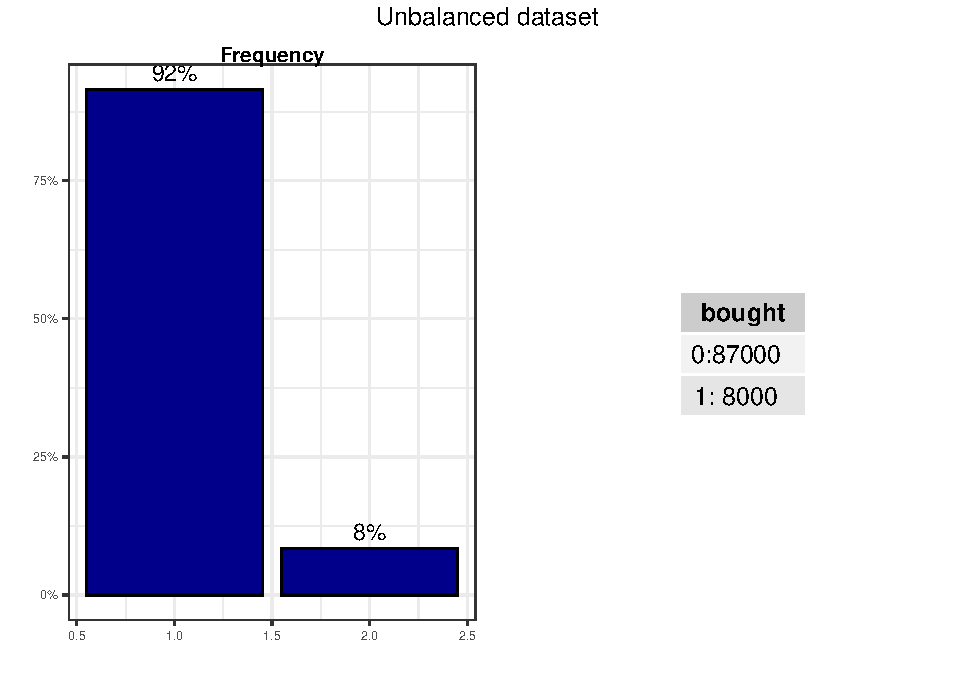
\includegraphics{_main_files/figure-latex/unnamed-chunk-11-1.pdf}

The ``bought'' variable is the target variable from this study and we can conclude the data is severely class inbalance towards no order which can affects modeling since it is biased towards the majority class. Has can be seen below this effect is corrected on the balanced dataset.

\begin{Shaded}
\begin{Highlighting}[]
\FunctionTok{grid.draw}\NormalTok{(balanced\_grid)}
\end{Highlighting}
\end{Shaded}

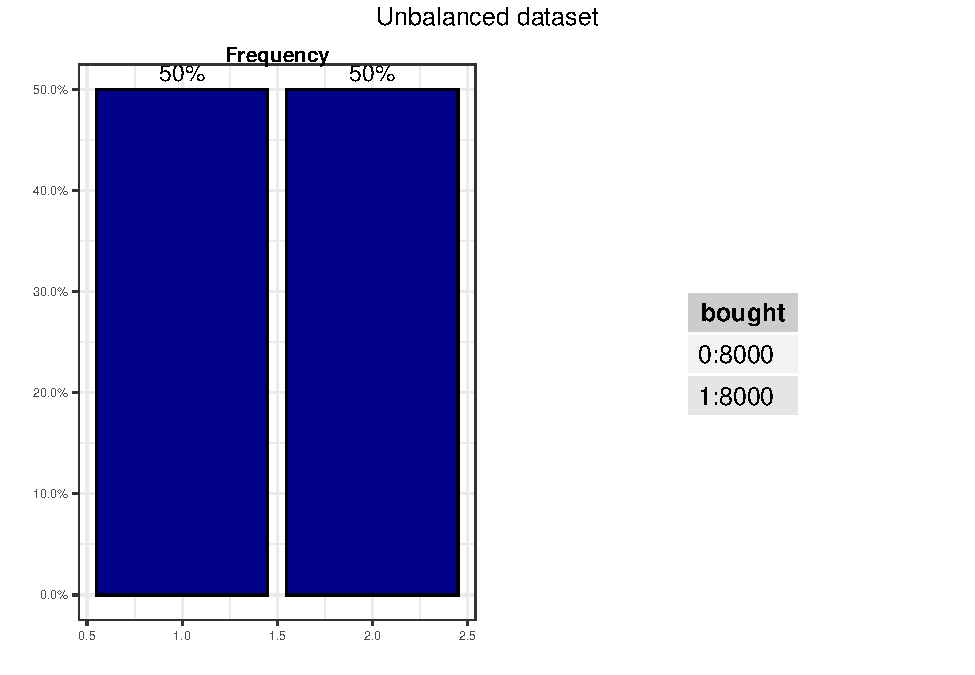
\includegraphics{_main_files/figure-latex/unnamed-chunk-12-1.pdf}

\hypertarget{customer-type}{%
\subsection{Customer type}\label{customer-type}}

\begin{Shaded}
\begin{Highlighting}[]
\FunctionTok{grid.draw}\NormalTok{(eda\_unbalanced}\SpecialCharTok{$}\NormalTok{customer\_type)}
\end{Highlighting}
\end{Shaded}

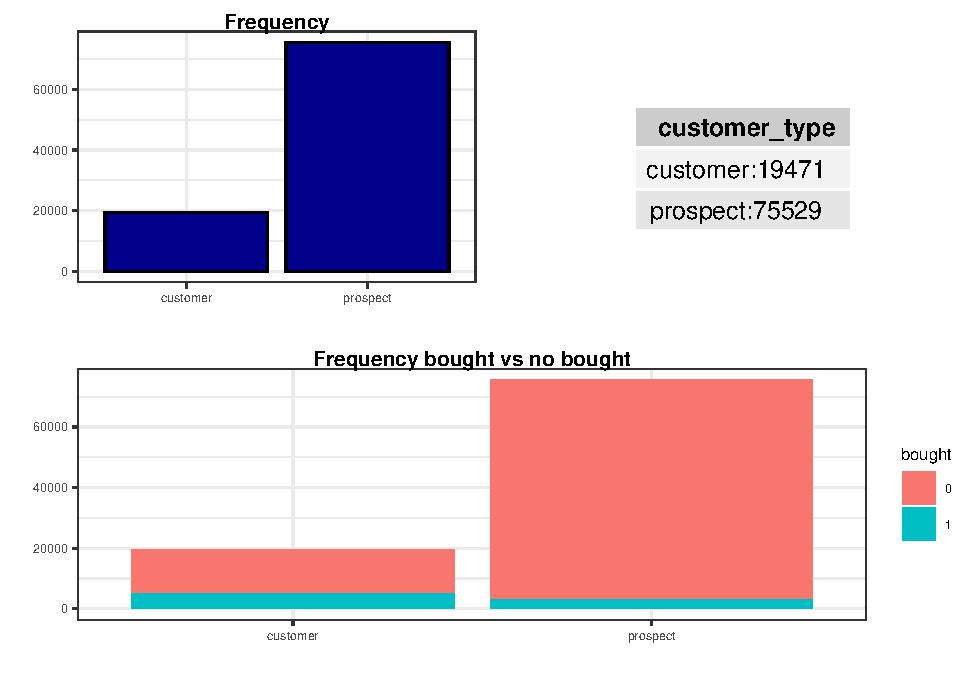
\includegraphics{_main_files/figure-latex/unnamed-chunk-13-1.pdf}

\begin{Shaded}
\begin{Highlighting}[]
\FunctionTok{grid.draw}\NormalTok{(eda\_unbalanced}\SpecialCharTok{$}\NormalTok{customer\_type)}
\end{Highlighting}
\end{Shaded}

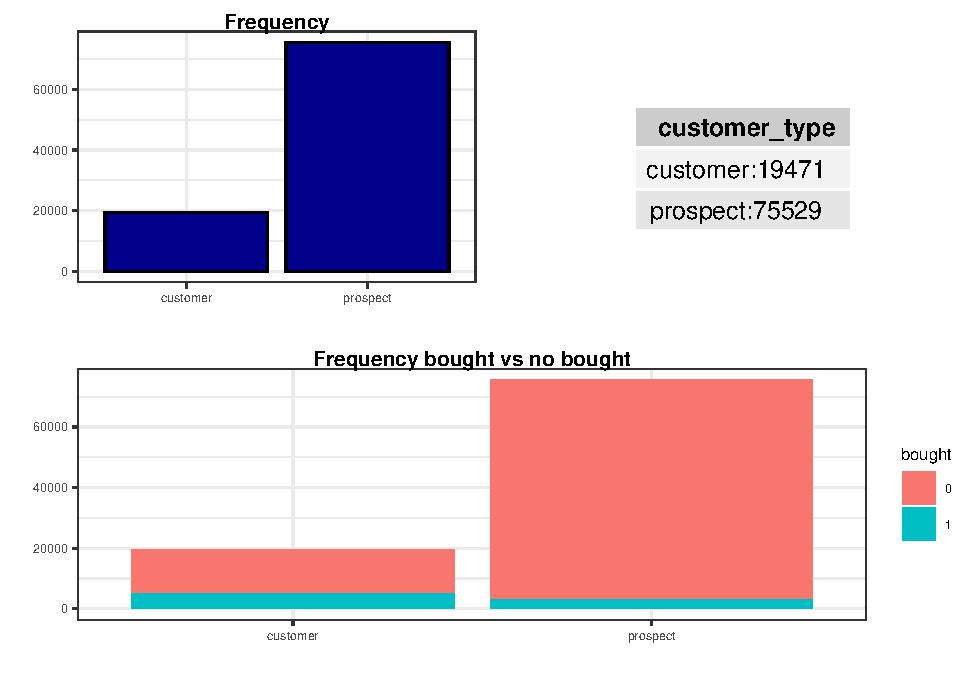
\includegraphics{_main_files/figure-latex/unnamed-chunk-14-1.pdf}

Customer type is a categorical variable with 2 levels. The current category in inbalanced with the majority of sessions being done by prospect clients. When compared with target the inbalanced differs slightly being bought the majority class for customers implying a relationship between the 2.

The resulst from the \(\chi^2\) hipotesis test does not refuse the null hipothesys reinforcing the graphical analysis that a relationship might exist between this 2 variables that implies that recurrent customers buy more.

\begin{Shaded}
\begin{Highlighting}[]
\NormalTok{unbalanced\_chi[}\StringTok{"customer\_type"}\NormalTok{]}
\end{Highlighting}
\end{Shaded}

\begin{verbatim}
## $customer_type
## 
##  Pearson's Chi-squared test with Yates' continuity correction
## 
## data:  x and unbalanced_data$bought
## X-squared = 9750.7, df = 1, p-value < 2.2e-16
\end{verbatim}

\begin{Shaded}
\begin{Highlighting}[]
\NormalTok{balanced\_chi[}\StringTok{"customer\_type"}\NormalTok{]}
\end{Highlighting}
\end{Shaded}

\begin{verbatim}
## $customer_type
## 
##  Pearson's Chi-squared test with Yates' continuity correction
## 
## data:  x and balanced_data$bought
## X-squared = 3590, df = 1, p-value < 2.2e-16
\end{verbatim}

\hypertarget{platform}{%
\subsection{Platform}\label{platform}}

\begin{Shaded}
\begin{Highlighting}[]
\FunctionTok{grid.draw}\NormalTok{(eda\_unbalanced}\SpecialCharTok{$}\NormalTok{platform)}
\end{Highlighting}
\end{Shaded}

\begin{Shaded}
\begin{Highlighting}[]
\FunctionTok{ggplot}\NormalTok{(unbalanced\_data, }\FunctionTok{aes}\NormalTok{(}\AttributeTok{x =}\NormalTok{ plaform)) }\SpecialCharTok{+}
    \FunctionTok{geom\_bar}\NormalTok{(}\AttributeTok{fill=}\StringTok{"darkblue"}\NormalTok{, }\AttributeTok{color=}\StringTok{"black"}\NormalTok{) }\SpecialCharTok{+}
    \FunctionTok{theme\_masterDS}\NormalTok{() }\SpecialCharTok{+}
    \FunctionTok{labs}\NormalTok{(}
      \AttributeTok{x =} \StringTok{""}\NormalTok{,}
      \AttributeTok{y =} \StringTok{""}\NormalTok{,}
      \AttributeTok{title =} \StringTok{"Frequency"}
\NormalTok{    )}
\end{Highlighting}
\end{Shaded}

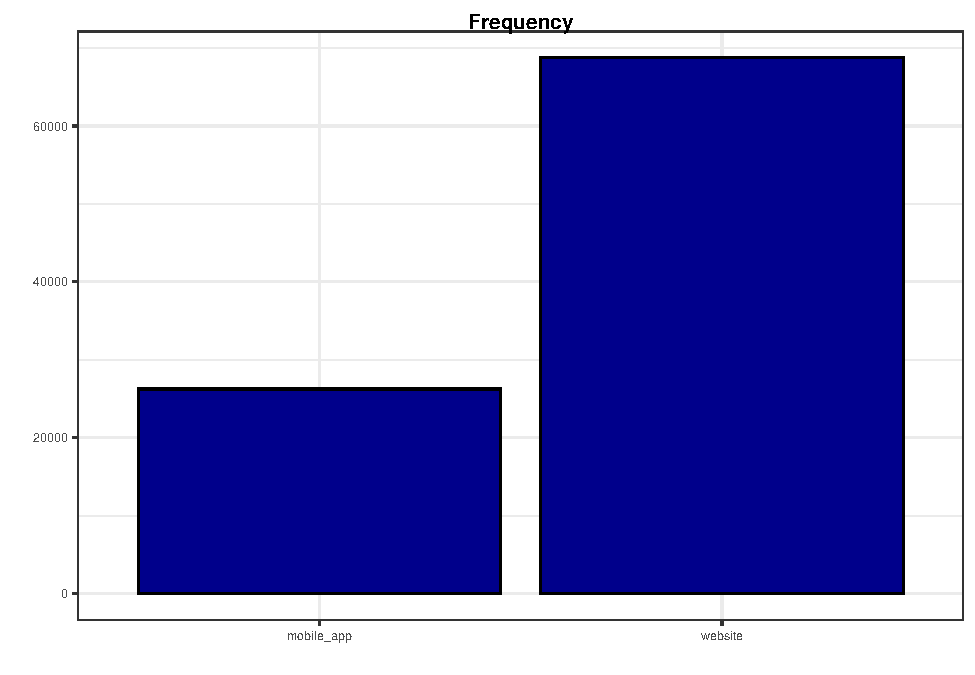
\includegraphics{_main_files/figure-latex/unnamed-chunk-18-1.pdf}

\begin{Shaded}
\begin{Highlighting}[]
\FunctionTok{ggplot}\NormalTok{(unbalanced\_data, }\FunctionTok{aes}\NormalTok{( }\AttributeTok{x =}\NormalTok{ plaform, }\AttributeTok{fill =}\NormalTok{ bought )) }\SpecialCharTok{+}
    \FunctionTok{geom\_bar}\NormalTok{() }\SpecialCharTok{+}
    \FunctionTok{theme\_masterDS}\NormalTok{() }\SpecialCharTok{+}
    \FunctionTok{labs}\NormalTok{(}
      \AttributeTok{x =} \StringTok{""}\NormalTok{,}
      \AttributeTok{y =} \StringTok{""}\NormalTok{,}
      \AttributeTok{title =} \StringTok{"Frequency bought vs no bought"}
\NormalTok{    )}
\end{Highlighting}
\end{Shaded}

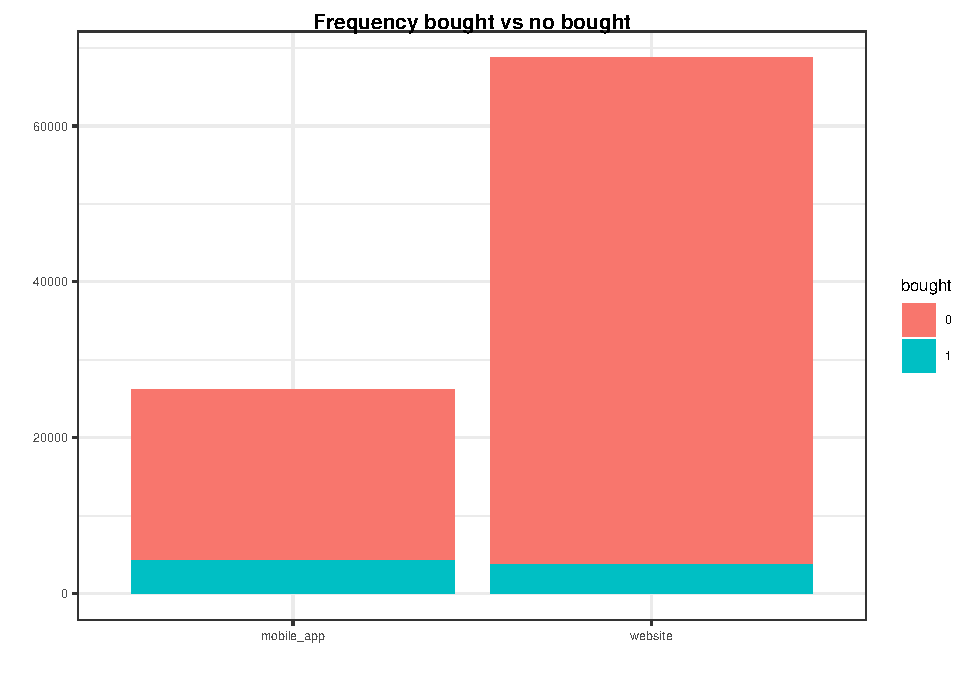
\includegraphics{_main_files/figure-latex/unnamed-chunk-19-1.pdf}

\begin{Shaded}
\begin{Highlighting}[]
\FunctionTok{prop.table}\NormalTok{(}\FunctionTok{table}\NormalTok{(unbalanced\_data[[}\StringTok{"plaform"}\NormalTok{]]))}
\end{Highlighting}
\end{Shaded}

\begin{verbatim}
## 
## mobile_app    website 
##  0.2761263  0.7238737
\end{verbatim}

\begin{Shaded}
\begin{Highlighting}[]
\NormalTok{unbalanced\_chi[}\StringTok{"plaform"}\NormalTok{]}
\end{Highlighting}
\end{Shaded}

\begin{verbatim}
## $plaform
## 
##  Pearson's Chi-squared test with Yates' continuity correction
## 
## data:  x and unbalanced_data$bought
## X-squared = 2896.4, df = 1, p-value < 2.2e-16
\end{verbatim}

\begin{Shaded}
\begin{Highlighting}[]
\FunctionTok{grid.draw}\NormalTok{(eda\_balanced}\SpecialCharTok{$}\NormalTok{platform)}
\end{Highlighting}
\end{Shaded}

\begin{Shaded}
\begin{Highlighting}[]
\FunctionTok{prop.table}\NormalTok{(}\FunctionTok{table}\NormalTok{(balanced\_data[[}\StringTok{"plaform"}\NormalTok{]]))}
\end{Highlighting}
\end{Shaded}

\begin{verbatim}
## 
## mobile_app    website 
##    0.39125    0.60875
\end{verbatim}

\begin{Shaded}
\begin{Highlighting}[]
\NormalTok{balanced\_chi[}\StringTok{"plaform"}\NormalTok{]}
\end{Highlighting}
\end{Shaded}

\begin{verbatim}
## $plaform
## 
##  Pearson's Chi-squared test with Yates' continuity correction
## 
## data:  x and balanced_data$bought
## X-squared = 1360.5, df = 1, p-value < 2.2e-16
\end{verbatim}

The graphical analysis show us that the majority of sessions (around 72\% on the unbalanced dataset and 61\% on the balanced ) were accessed through the website. Despite the inbalance between platforms we notice that the amount of conversion is comparable suggesting implying a higher conversion rate on mobile app compared to website.

The \(\chi ^2\) for both unbalanced and balanced datasets do not allow for the rejection of the null hypothesis implying the existence of a degree of linear regression between the 2 variables.

\hypertarget{segment}{%
\subsection{Segment}\label{segment}}

\begin{Shaded}
\begin{Highlighting}[]
\FunctionTok{grid.draw}\NormalTok{(eda\_unbalanced}\SpecialCharTok{$}\NormalTok{segment)}
\end{Highlighting}
\end{Shaded}

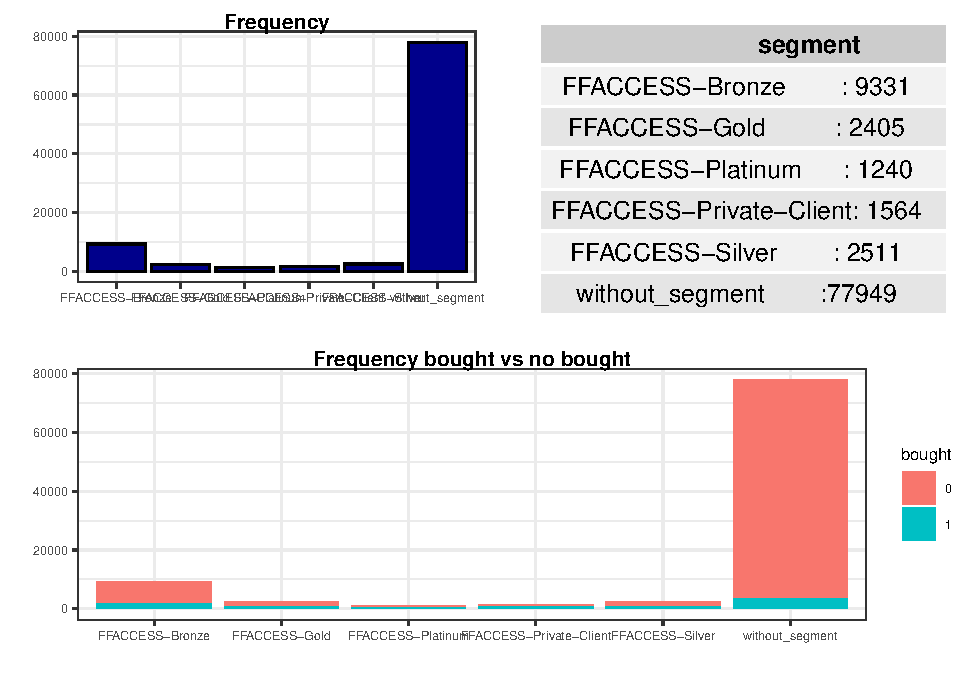
\includegraphics{_main_files/figure-latex/unnamed-chunk-25-1.pdf}

\begin{Shaded}
\begin{Highlighting}[]
\NormalTok{unbalanced\_chi[}\StringTok{"segment"}\NormalTok{]}
\end{Highlighting}
\end{Shaded}

\begin{verbatim}
## $segment
## 
##  Pearson's Chi-squared test
## 
## data:  x and unbalanced_data$bought
## X-squared = 10203, df = 5, p-value < 2.2e-16
\end{verbatim}

\begin{Shaded}
\begin{Highlighting}[]
\FunctionTok{grid.draw}\NormalTok{(eda\_balanced}\SpecialCharTok{$}\NormalTok{segment)}
\end{Highlighting}
\end{Shaded}

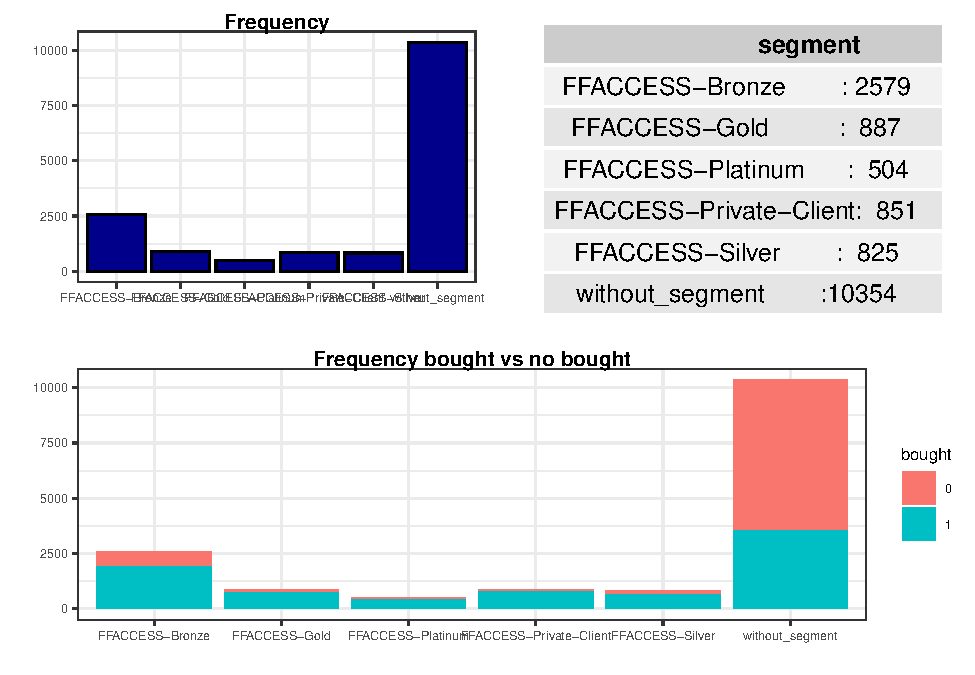
\includegraphics{_main_files/figure-latex/unnamed-chunk-27-1.pdf}

\begin{Shaded}
\begin{Highlighting}[]
\NormalTok{balanced\_chi[}\StringTok{"segment"}\NormalTok{]}
\end{Highlighting}
\end{Shaded}

\begin{verbatim}
## $segment
## 
##  Pearson's Chi-squared test
## 
## data:  x and balanced_data$bought
## X-squared = 3071, df = 5, p-value < 2.2e-16
\end{verbatim}

The graphical analysis shows that the great majority of sessions were executed by users not belonging to any segment. Does not point to any relationship. The \(\chi ^2\) test for both unbalanced and balanced datasets do not allow for the rejection of the null hypothesis implying the existence of a degree of linear regression between the 2 variables.

\hypertarget{device-group}{%
\subsection{Device Group}\label{device-group}}

\begin{Shaded}
\begin{Highlighting}[]
\FunctionTok{grid.draw}\NormalTok{(eda\_unbalanced}\SpecialCharTok{$}\NormalTok{device\_group)}
\end{Highlighting}
\end{Shaded}

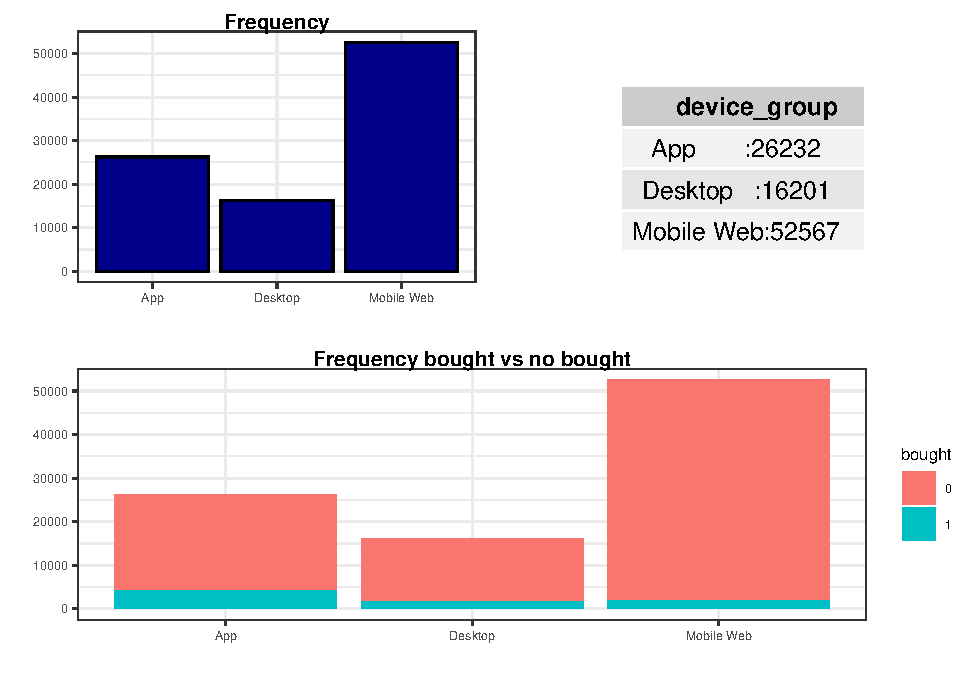
\includegraphics{_main_files/figure-latex/unnamed-chunk-29-1.pdf}

\begin{Shaded}
\begin{Highlighting}[]
\NormalTok{unbalanced\_chi[}\StringTok{"device\_group"}\NormalTok{]}
\end{Highlighting}
\end{Shaded}

\begin{verbatim}
## $device_group
## 
##  Pearson's Chi-squared test
## 
## data:  x and unbalanced_data$bought
## X-squared = 3755.4, df = 2, p-value < 2.2e-16
\end{verbatim}

\begin{Shaded}
\begin{Highlighting}[]
\FunctionTok{grid.draw}\NormalTok{(eda\_balanced}\SpecialCharTok{$}\NormalTok{device\_group)}
\end{Highlighting}
\end{Shaded}

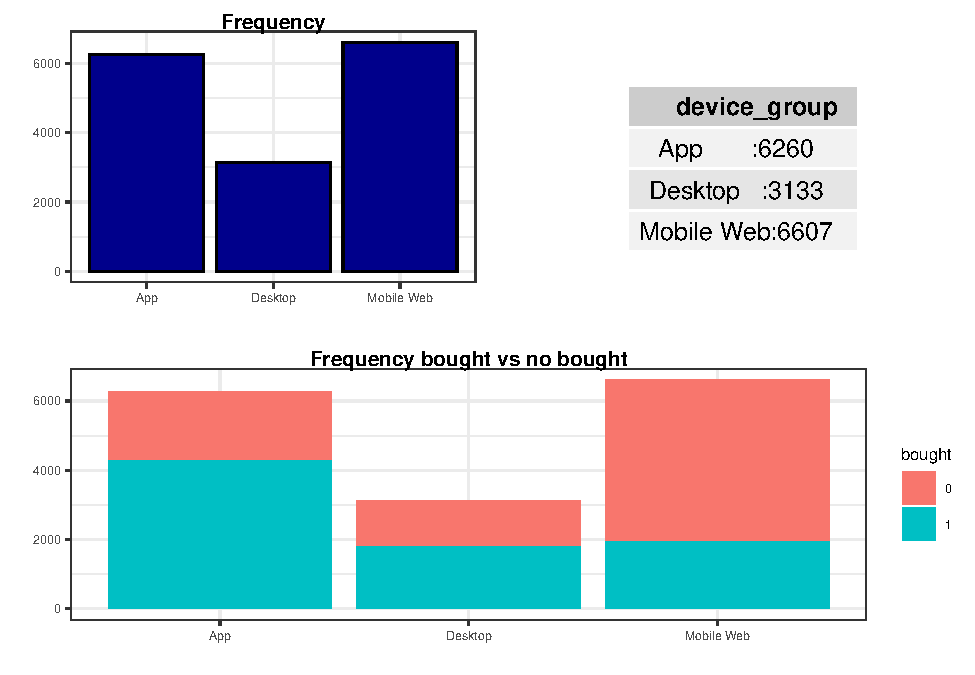
\includegraphics{_main_files/figure-latex/unnamed-chunk-31-1.pdf}

\begin{Shaded}
\begin{Highlighting}[]
\NormalTok{balanced\_chi[}\StringTok{"device\_group"}\NormalTok{]}
\end{Highlighting}
\end{Shaded}

\begin{verbatim}
## $device_group
## 
##  Pearson's Chi-squared test
## 
## data:  x and balanced_data$bought
## X-squared = 2003.4, df = 2, p-value < 2.2e-16
\end{verbatim}

The graphical analysis of the data tells us that the majority of sessions have been done using Mobile Web platform, although, when taking into account the actual conversion it suggests that a higher conversion rate exists on application or desktop than compared with Majority class.

This same conclusions can be extracted from the balanced dataset although the differences are not as evident. The \(\chi ^2\) tests for both dataset leads into refusing the null hypothesis so it suggests that a degree of relation ship exists between both variables.

\begin{Shaded}
\begin{Highlighting}[]
\FunctionTok{ggplot}\NormalTok{(unbalanced\_data, }\FunctionTok{aes}\NormalTok{(}\AttributeTok{x =}\NormalTok{ device\_group, }\AttributeTok{fill =}\NormalTok{ plaform)) }\SpecialCharTok{+} 
  \FunctionTok{geom\_bar}\NormalTok{(}\AttributeTok{stat =} \StringTok{"count"}\NormalTok{) }\SpecialCharTok{+} 
  \FunctionTok{theme\_masterDS}\NormalTok{() }\SpecialCharTok{+}
    \FunctionTok{labs}\NormalTok{(}
      \AttributeTok{x =} \StringTok{""}\NormalTok{,}
      \AttributeTok{y =} \StringTok{""}\NormalTok{,}
      \AttributeTok{title =} \StringTok{"Device Group x Platform"}
\NormalTok{    )}
\end{Highlighting}
\end{Shaded}

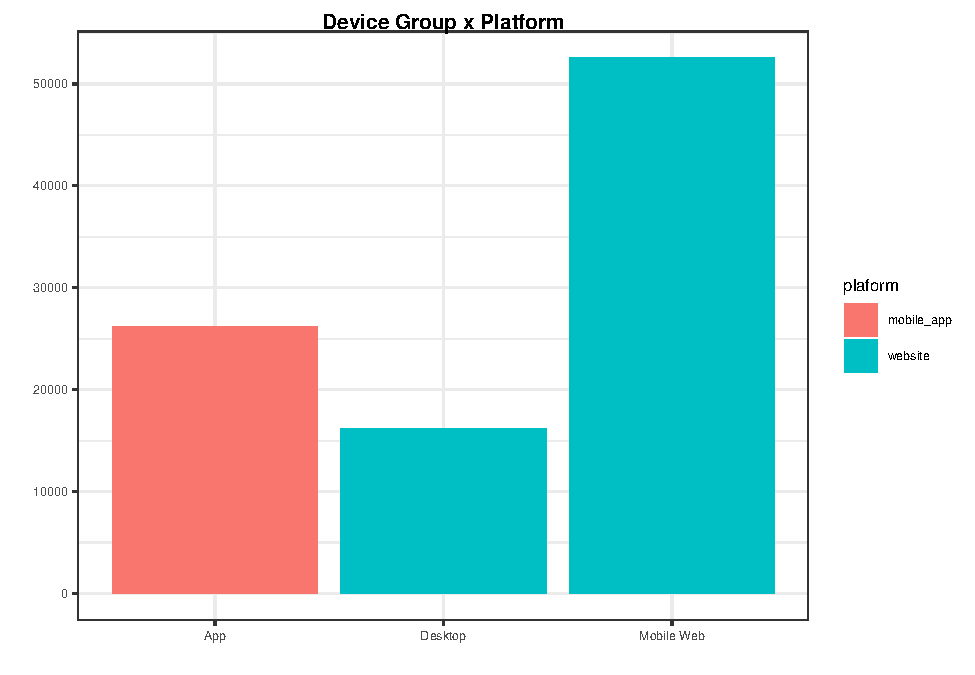
\includegraphics{_main_files/figure-latex/unnamed-chunk-33-1.pdf}

This dataset includes a variable named platform that suggest that most sessions were done using website. At first glance it seems counter intuitive that most access be done through website and Mobile web but the above plot show that in reality most users opt to access using the mobile version of the website instead of the app.

The \(\chi ^2\) test between this 2 variables confirms what we could already suspect from visual inspection, both variable seem to have a degree of relation leading to not refuting the null hiopothesis of dependeny. This implies interaction (or sinergy on marketing terms) between features which can impact how modeling efforts specially for models dependent on linear transformations (least squares regression) as is the case of logit.

During the modeling step one might consider removing one of the variables or generate a new compound feature.

\begin{Shaded}
\begin{Highlighting}[]
\FunctionTok{chisq.test}\NormalTok{(}\FunctionTok{as.character}\NormalTok{(unbalanced\_data}\SpecialCharTok{$}\NormalTok{plaform), }\FunctionTok{as.character}\NormalTok{(unbalanced\_data}\SpecialCharTok{$}\NormalTok{device\_group))}
\end{Highlighting}
\end{Shaded}

\begin{verbatim}
## 
##  Pearson's Chi-squared test
## 
## data:  as.character(unbalanced_data$plaform) and as.character(unbalanced_data$device_group)
## X-squared = 95000, df = 2, p-value < 2.2e-16
\end{verbatim}

\hypertarget{visitor-type}{%
\subsection{Visitor type}\label{visitor-type}}

\begin{Shaded}
\begin{Highlighting}[]
\FunctionTok{grid.draw}\NormalTok{(eda\_unbalanced}\SpecialCharTok{$}\NormalTok{visitor\_type)}
\end{Highlighting}
\end{Shaded}

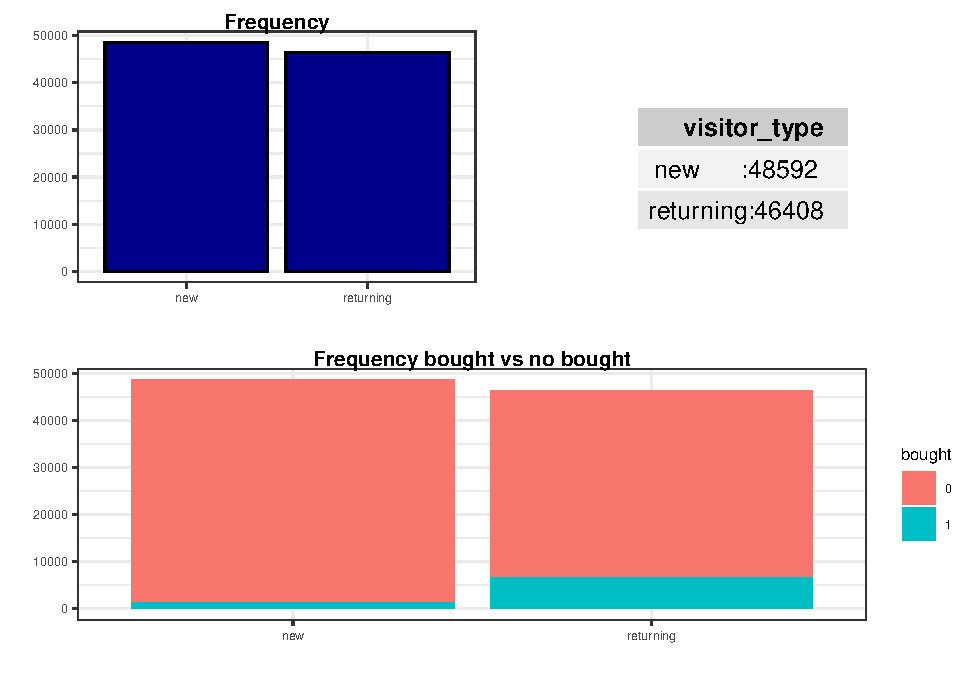
\includegraphics{_main_files/figure-latex/unnamed-chunk-35-1.pdf}

\begin{Shaded}
\begin{Highlighting}[]
\NormalTok{unbalanced\_chi[}\StringTok{"visitor\_type"}\NormalTok{]}
\end{Highlighting}
\end{Shaded}

\begin{verbatim}
## $visitor_type
## 
##  Pearson's Chi-squared test with Yates' continuity correction
## 
## data:  x and unbalanced_data$bought
## X-squared = 4001.3, df = 1, p-value < 2.2e-16
\end{verbatim}

\begin{Shaded}
\begin{Highlighting}[]
\FunctionTok{grid.draw}\NormalTok{(eda\_balanced}\SpecialCharTok{$}\NormalTok{visitor\_type)}
\end{Highlighting}
\end{Shaded}

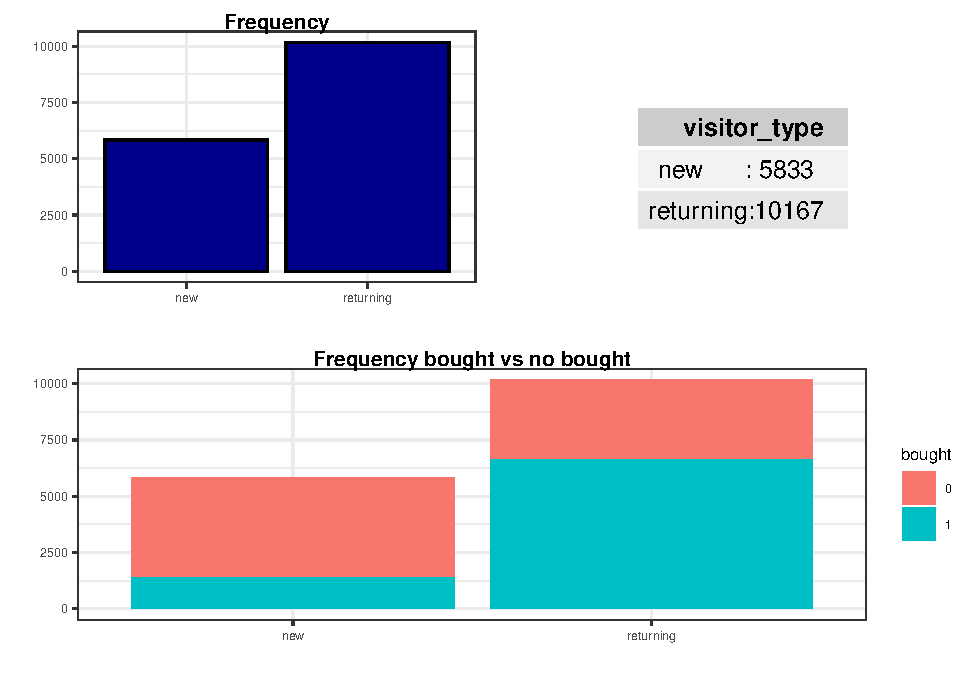
\includegraphics{_main_files/figure-latex/unnamed-chunk-37-1.pdf}

\begin{Shaded}
\begin{Highlighting}[]
\NormalTok{balanced\_chi[}\StringTok{"visitor\_type"}\NormalTok{]}
\end{Highlighting}
\end{Shaded}

\begin{verbatim}
## $visitor_type
## 
##  Pearson's Chi-squared test with Yates' continuity correction
## 
## data:  x and balanced_data$bought
## X-squared = 2529.6, df = 1, p-value < 2.2e-16
\end{verbatim}

This feature focus on the Visitors. The unbalanced data available shows almost a 50\% split, situations that changes on the balanced dataset which has a inbalance towards returning visitors. The graphical analysis suggests a higher conversion rate for returning visitor that for new one, suggesting that continuous visits (engagment) plays a role in conversion.

The current dataset has information regarding customer type crossed with visitor type can provide us with interesting information

\begin{Shaded}
\begin{Highlighting}[]
\FunctionTok{ggplot}\NormalTok{(unbalanced\_data, }\FunctionTok{aes}\NormalTok{(}\AttributeTok{x =}\NormalTok{ visitor\_type, }\AttributeTok{fill =}\NormalTok{ customer\_type)) }\SpecialCharTok{+} 
  \FunctionTok{geom\_bar}\NormalTok{(}\AttributeTok{stat =} \StringTok{"count"}\NormalTok{) }\SpecialCharTok{+} 
  \FunctionTok{theme\_masterDS}\NormalTok{() }\SpecialCharTok{+}
    \FunctionTok{labs}\NormalTok{(}
      \AttributeTok{x =} \StringTok{""}\NormalTok{,}
      \AttributeTok{y =} \StringTok{""}\NormalTok{,}
      \AttributeTok{title =} \StringTok{"Visitor Type x Custor Type"}
\NormalTok{    )}
\end{Highlighting}
\end{Shaded}

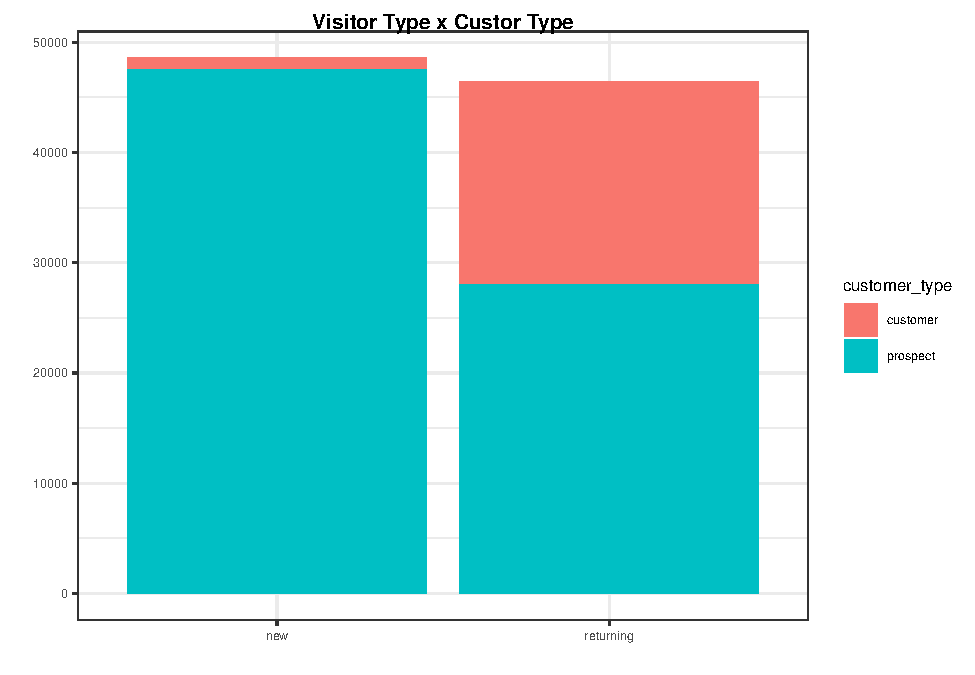
\includegraphics{_main_files/figure-latex/unnamed-chunk-39-1.pdf}

Has expected only a fraction of new visitors actually buy on the first session hinting that the conversion journey is longer than one session, meaning than several visits are needed before a first conversion. We don't have enough information to conclude about the number of sessions needed (journey lenght) and neither the session index given a time window (eg: the current session is the \#3 in the last 28 days) which is know to have a impact on conversion.

\hypertarget{journey-milestones}{%
\subsection{Journey milestones}\label{journey-milestones}}

(has\_listings) \textgreater{} has\_add\_to\_bag

\begin{Shaded}
\begin{Highlighting}[]
\FunctionTok{grid.draw}\NormalTok{(eda\_unbalanced}\SpecialCharTok{$}\NormalTok{has\_add\_to\_wishlist)}
\end{Highlighting}
\end{Shaded}

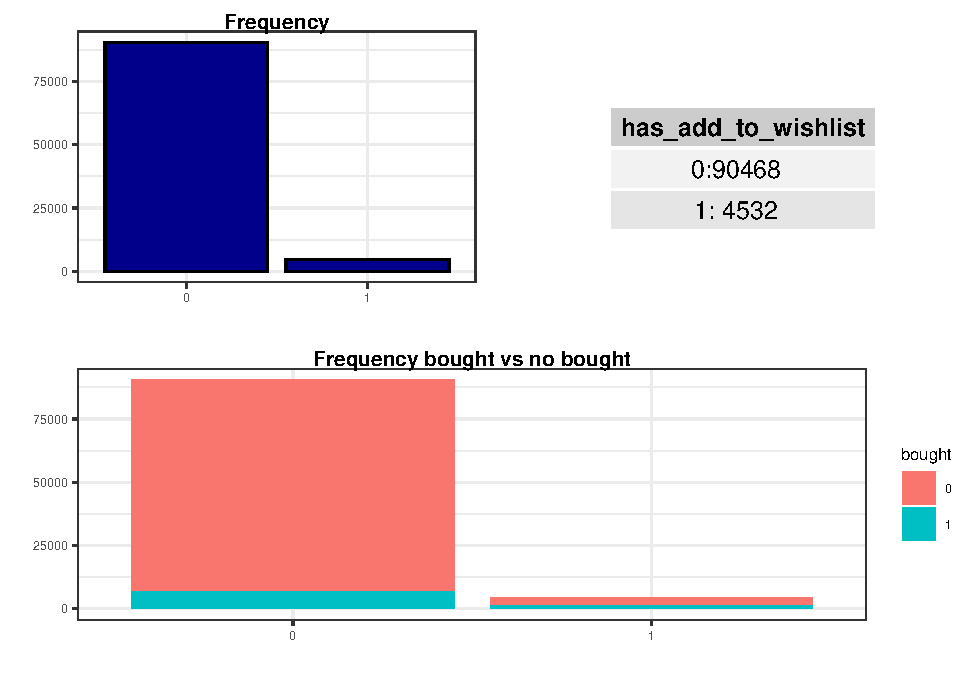
\includegraphics{_main_files/figure-latex/unnamed-chunk-40-1.pdf}

\begin{Shaded}
\begin{Highlighting}[]
\FunctionTok{grid.draw}\NormalTok{(eda\_unbalanced}\SpecialCharTok{$}\NormalTok{has\_listing)}
\end{Highlighting}
\end{Shaded}

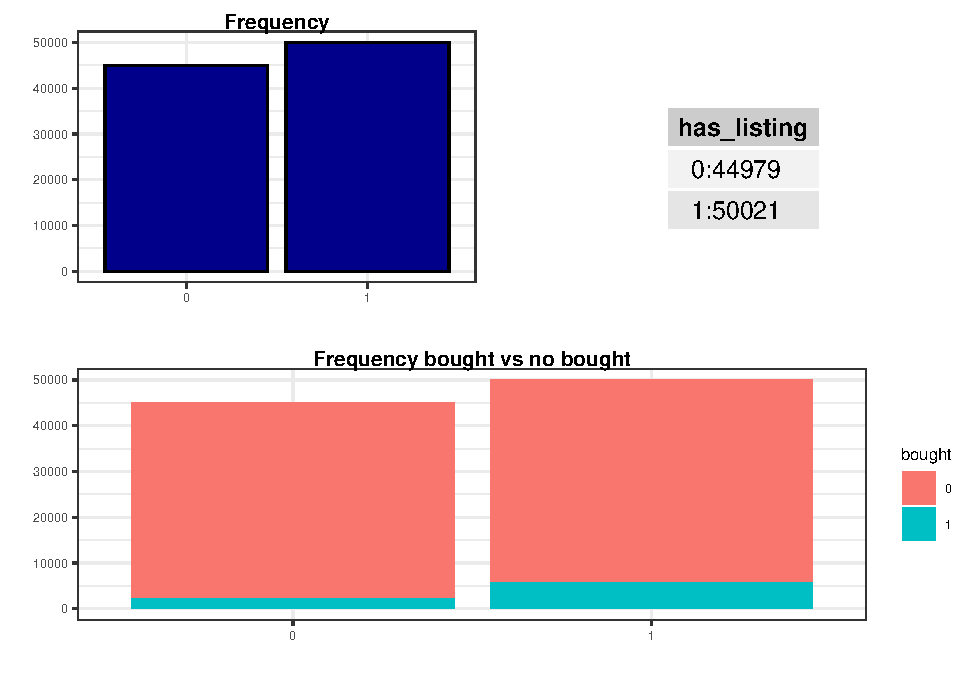
\includegraphics{_main_files/figure-latex/unnamed-chunk-41-1.pdf}

\begin{Shaded}
\begin{Highlighting}[]
\FunctionTok{grid.draw}\NormalTok{(eda\_unbalanced}\SpecialCharTok{$}\NormalTok{has\_recommendation)}
\end{Highlighting}
\end{Shaded}

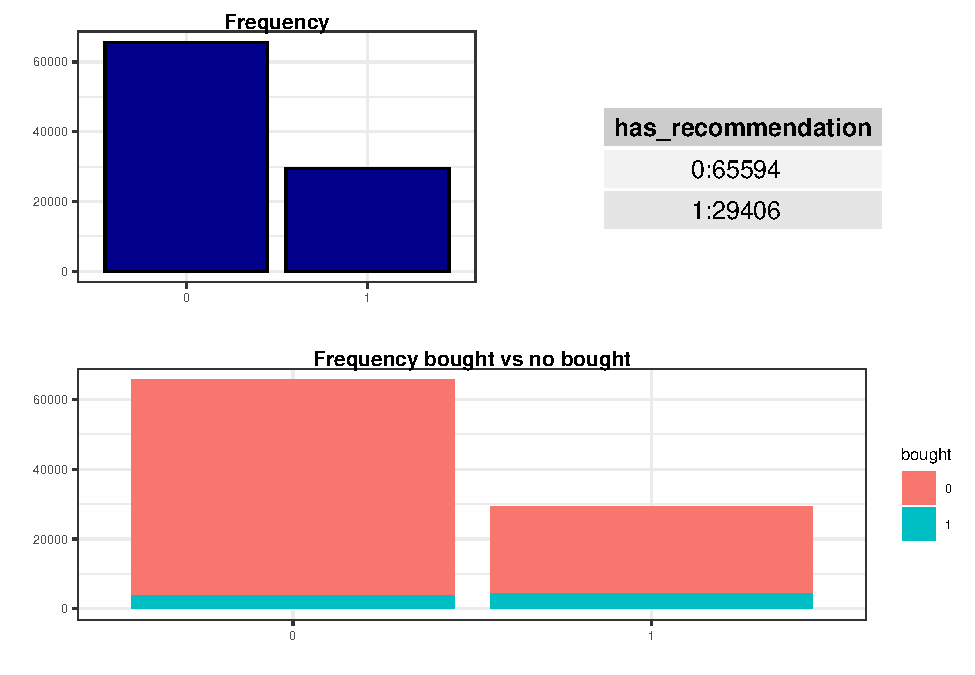
\includegraphics{_main_files/figure-latex/unnamed-chunk-42-1.pdf}

\begin{Shaded}
\begin{Highlighting}[]
\FunctionTok{grid.draw}\NormalTok{(eda\_unbalanced}\SpecialCharTok{$}\NormalTok{has\_used\_search)}
\end{Highlighting}
\end{Shaded}

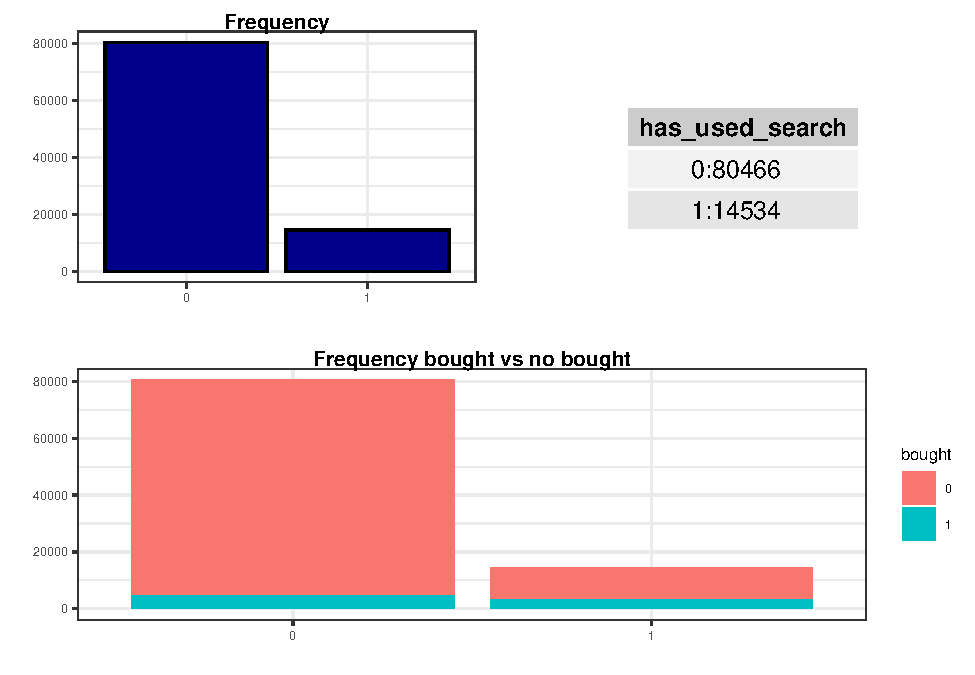
\includegraphics{_main_files/figure-latex/unnamed-chunk-43-1.pdf}

\begin{Shaded}
\begin{Highlighting}[]
\FunctionTok{grid.draw}\NormalTok{(eda\_unbalanced}\SpecialCharTok{$}\NormalTok{has\_add\_to\_bag)}
\end{Highlighting}
\end{Shaded}

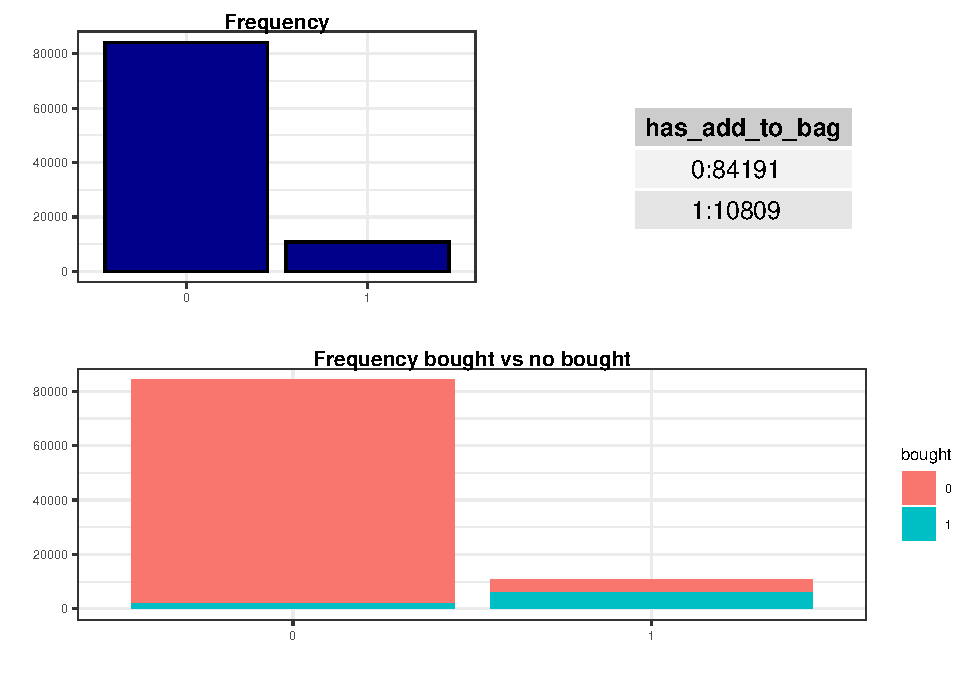
\includegraphics{_main_files/figure-latex/unnamed-chunk-44-1.pdf}

This features are plotted together because they give insights into the journey a user made inside the website. We can conclude over a conversion funnel but it makes sense to explore the interactions between then while modeling because its known that normally strong effects exist between then (a user had a recommendation and added to the bag might be together a strong signal for conversion).

The graphical analysis already provides a important insight given the business objectives. From the unbalanced data available we can conclude that around of 46\% shopping carts are lost on that session. That raises a question of how are this recovered (example on a next session) or if this means that all this sales are lost right at the end of the sales funnel.

\begin{Shaded}
\begin{Highlighting}[]
\FunctionTok{prop.table}\NormalTok{(}\FunctionTok{table}\NormalTok{(unbalanced\_data[unbalanced\_data}\SpecialCharTok{$}\NormalTok{has\_add\_to\_bag }\SpecialCharTok{==} \DecValTok{1}\NormalTok{,]}\SpecialCharTok{$}\NormalTok{bought, unbalanced\_data[unbalanced\_data}\SpecialCharTok{$}\NormalTok{has\_add\_to\_bag }\SpecialCharTok{==} \DecValTok{1}\NormalTok{,]}\SpecialCharTok{$}\NormalTok{has\_add\_to\_bag)) [,}\DecValTok{2}\NormalTok{]}
\end{Highlighting}
\end{Shaded}

\begin{verbatim}
##         0         1 
## 0.4500879 0.5499121
\end{verbatim}

\hypertarget{duration}{%
\subsection{Duration}\label{duration}}

\begin{Shaded}
\begin{Highlighting}[]
\FunctionTok{grid.draw}\NormalTok{(eda\_unbalanced}\SpecialCharTok{$}\NormalTok{duration) }
\end{Highlighting}
\end{Shaded}

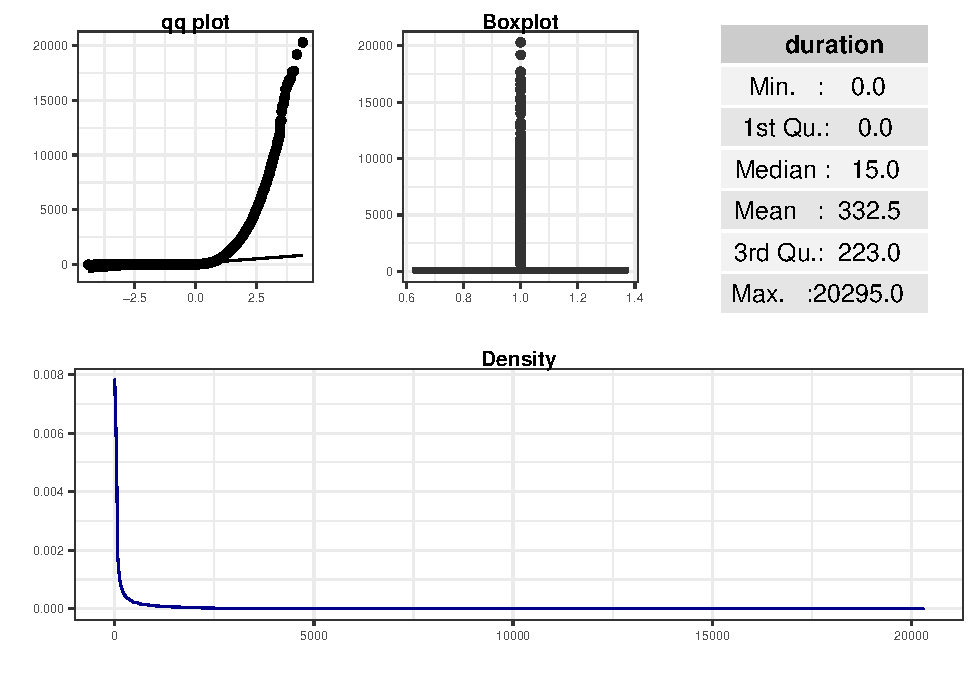
\includegraphics{_main_files/figure-latex/unnamed-chunk-46-1.pdf}

\begin{Shaded}
\begin{Highlighting}[]
\FunctionTok{grid.draw}\NormalTok{(eda\_balanced}\SpecialCharTok{$}\NormalTok{duration) }
\end{Highlighting}
\end{Shaded}

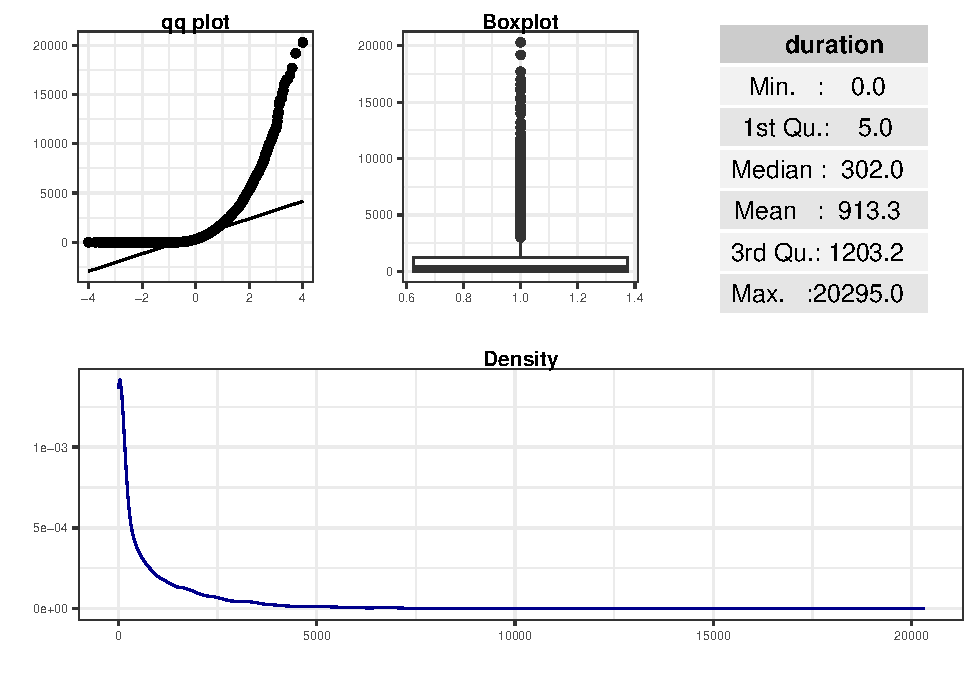
\includegraphics{_main_files/figure-latex/unnamed-chunk-47-1.pdf}

Both unbalanced and balanced datasets show a left skewed distribution for duration. The Distance between the Mean and Median provides a good view of data. This extrem values have a big influence impacting the gaussianity of the distribution.

Normally web analytics software limit session duration between 25 to 30 min. It is assumed that beyond that point either the user is idle or there is a error on the collection. For periods of engagement superior to that cap normally a new session is started. So a 1hour of engagement would signify 2 simultaneous sessions.

In the case of our project we have no context regarding session duration. Therefore, we have no referencial from business which would lead us to remove.

From the graphical view we can see that the variable distribution is left skewed whcih can cause us problems during modeling and impacts our outlier analysis. We will log transform this variable.

\begin{Shaded}
\begin{Highlighting}[]
\NormalTok{up }\OtherTok{\textless{}{-}} \FunctionTok{quantile}\NormalTok{(unbalanced\_data}\SpecialCharTok{$}\NormalTok{duration, }\FloatTok{0.75}\NormalTok{) }\SpecialCharTok{+} \DecValTok{3} \SpecialCharTok{*} \FunctionTok{IQR}\NormalTok{(unbalanced\_data}\SpecialCharTok{$}\NormalTok{duration)}

\NormalTok{unbalanced\_outlier\_clean }\OtherTok{\textless{}{-}}\NormalTok{ unbalanced\_data }\SpecialCharTok{\%\textgreater{}\%} 
  \FunctionTok{filter}\NormalTok{(duration }\SpecialCharTok{\textless{}}\NormalTok{ up) }

\NormalTok{  density }\OtherTok{\textless{}{-}} \FunctionTok{ggplot}\NormalTok{(unbalanced\_data, }\FunctionTok{aes}\NormalTok{(}\AttributeTok{x =}\NormalTok{ duration)) }\SpecialCharTok{+}
    \FunctionTok{geom\_density}\NormalTok{(}\AttributeTok{color=}\StringTok{"darkblue"}\NormalTok{) }\SpecialCharTok{+}
    \FunctionTok{theme\_masterDS}\NormalTok{() }\SpecialCharTok{+}
    \FunctionTok{labs}\NormalTok{(}
      \AttributeTok{x =} \StringTok{""}\NormalTok{,}
      \AttributeTok{y =} \StringTok{""}\NormalTok{,}
      \AttributeTok{title =} \StringTok{"Density"}
\NormalTok{    )}
  
\NormalTok{  boxplot }\OtherTok{\textless{}{-}} \FunctionTok{ggplot}\NormalTok{(unbalanced\_data, }\FunctionTok{aes}\NormalTok{(}\AttributeTok{x =} \DecValTok{1}\NormalTok{, }\AttributeTok{y =}\NormalTok{ duration)) }\SpecialCharTok{+} 
    \FunctionTok{geom\_boxplot}\NormalTok{() }\SpecialCharTok{+} 
    \FunctionTok{theme\_masterDS}\NormalTok{()}\SpecialCharTok{+}
    \FunctionTok{labs}\NormalTok{(}
      \AttributeTok{x =} \StringTok{""}\NormalTok{,}
      \AttributeTok{y=}\StringTok{""}\NormalTok{,}
      \AttributeTok{title =} \StringTok{"Boxplot"}
\NormalTok{    )   }

\NormalTok{  density\_log }\OtherTok{\textless{}{-}} \FunctionTok{ggplot}\NormalTok{(unbalanced\_data, }\FunctionTok{aes}\NormalTok{(}\AttributeTok{x =} \FunctionTok{log}\NormalTok{(duration))) }\SpecialCharTok{+}
    \FunctionTok{geom\_density}\NormalTok{(}\AttributeTok{color=}\StringTok{"darkblue"}\NormalTok{) }\SpecialCharTok{+}
    \FunctionTok{theme\_masterDS}\NormalTok{() }\SpecialCharTok{+}
    \FunctionTok{labs}\NormalTok{(}
      \AttributeTok{x =} \StringTok{""}\NormalTok{,}
      \AttributeTok{y =} \StringTok{""}\NormalTok{,}
      \AttributeTok{title =} \StringTok{"Density (log transform)"}
\NormalTok{    )}
  
\NormalTok{  boxplot\_log }\OtherTok{\textless{}{-}} \FunctionTok{ggplot}\NormalTok{(unbalanced\_data, }\FunctionTok{aes}\NormalTok{(}\AttributeTok{x =} \DecValTok{1}\NormalTok{, }\AttributeTok{y =} \FunctionTok{log}\NormalTok{(duration))) }\SpecialCharTok{+} 
    \FunctionTok{geom\_boxplot}\NormalTok{() }\SpecialCharTok{+} 
    \FunctionTok{theme\_masterDS}\NormalTok{()}\SpecialCharTok{+}
    \FunctionTok{labs}\NormalTok{(}
      \AttributeTok{x =} \StringTok{""}\NormalTok{,}
      \AttributeTok{y=}\StringTok{""}\NormalTok{,}
      \AttributeTok{title =} \StringTok{"Boxplot (log trasnform)"}
\NormalTok{    ) }

\FunctionTok{grid.arrange}\NormalTok{(density, boxplot, density\_log, boxplot\_log,  }\AttributeTok{layout\_matrix =} \FunctionTok{rbind}\NormalTok{(}\FunctionTok{c}\NormalTok{(}\DecValTok{1}\NormalTok{,}\DecValTok{2}\NormalTok{),}\FunctionTok{c}\NormalTok{(}\DecValTok{3}\NormalTok{,}\DecValTok{4}\NormalTok{)))}
\end{Highlighting}
\end{Shaded}

\begin{verbatim}
## Warning: Removed 41417 rows containing non-finite values (stat_density).
\end{verbatim}

\begin{verbatim}
## Warning: Removed 41417 rows containing non-finite values (stat_boxplot).
\end{verbatim}

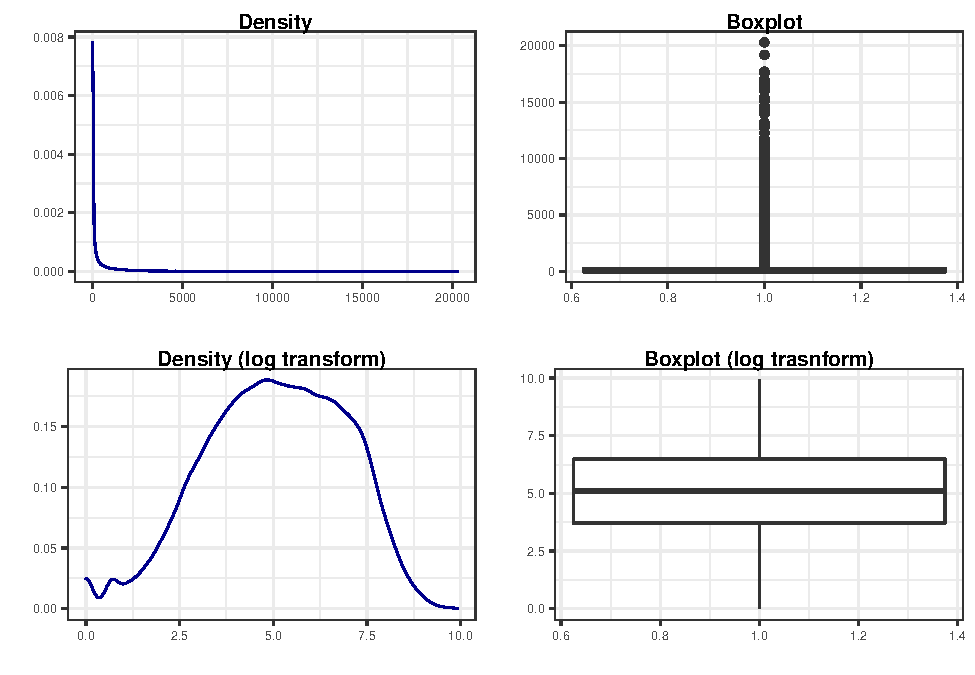
\includegraphics{_main_files/figure-latex/unnamed-chunk-48-1.pdf}

\hypertarget{view-quantity}{%
\subsection{View quantity}\label{view-quantity}}

\begin{Shaded}
\begin{Highlighting}[]
\FunctionTok{grid.draw}\NormalTok{(eda\_unbalanced}\SpecialCharTok{$}\NormalTok{view\_qty)}
\end{Highlighting}
\end{Shaded}

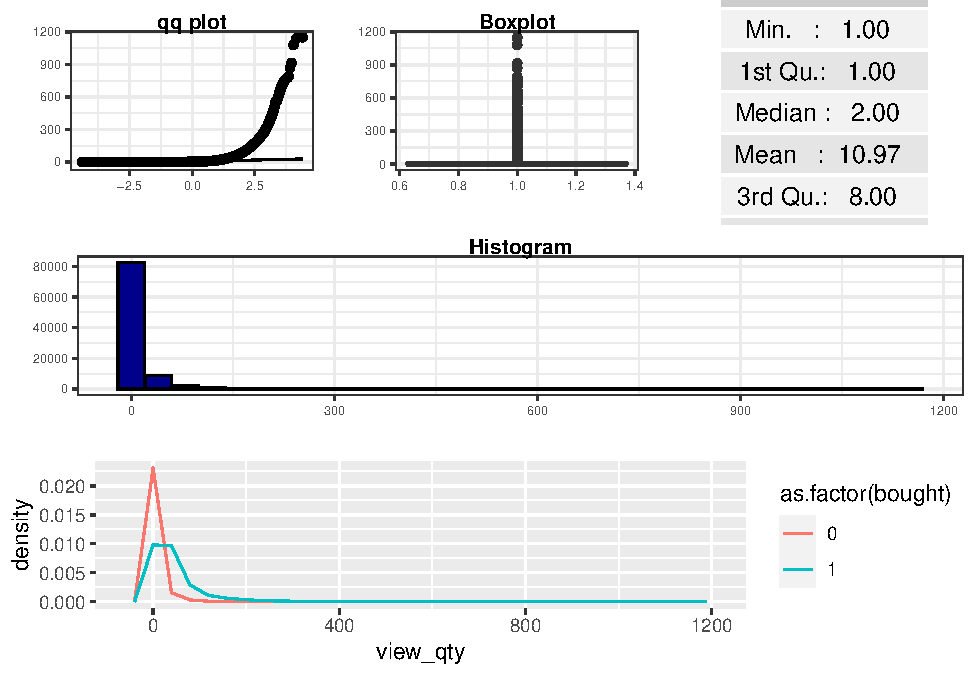
\includegraphics{_main_files/figure-latex/unnamed-chunk-49-1.pdf}

\begin{Shaded}
\begin{Highlighting}[]
\FunctionTok{grid.draw}\NormalTok{(eda\_balanced}\SpecialCharTok{$}\NormalTok{view\_qty)}
\end{Highlighting}
\end{Shaded}

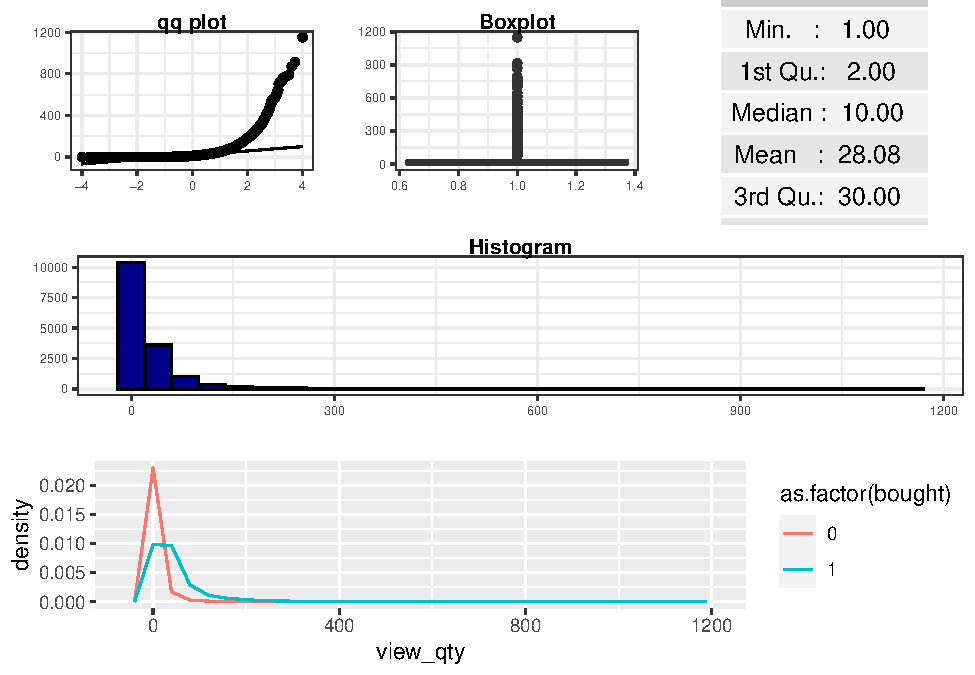
\includegraphics{_main_files/figure-latex/unnamed-chunk-50-1.pdf}

left skwed apply log transform

\begin{Shaded}
\begin{Highlighting}[]
\NormalTok{ lambda }\OtherTok{\textless{}{-}} \FunctionTok{BoxCox.lambda}\NormalTok{(unbalanced\_data}\SpecialCharTok{$}\NormalTok{view\_qty, }\AttributeTok{method =} \StringTok{"guerrero"}\NormalTok{) }

\NormalTok{histogram\_log }\OtherTok{\textless{}{-}} \FunctionTok{ggplot}\NormalTok{(unbalanced\_data, }\FunctionTok{aes}\NormalTok{(}\AttributeTok{x =} \FunctionTok{bcPower}\NormalTok{(view\_qty, }\AttributeTok{lambda =}\NormalTok{ lambda))) }\SpecialCharTok{+}
    \FunctionTok{geom\_histogram}\NormalTok{(}\AttributeTok{fill=}\StringTok{"darkblue"}\NormalTok{, }\AttributeTok{color=}\StringTok{"black"}\NormalTok{) }\SpecialCharTok{+}
    \FunctionTok{theme\_masterDS}\NormalTok{() }\SpecialCharTok{+}
    \FunctionTok{labs}\NormalTok{(}
      \AttributeTok{x =} \StringTok{""}\NormalTok{,}
      \AttributeTok{y =} \StringTok{""}\NormalTok{,}
      \AttributeTok{title =} \StringTok{"Histogram"}
\NormalTok{    )}
  
\NormalTok{  boxplot\_log }\OtherTok{\textless{}{-}} \FunctionTok{ggplot}\NormalTok{(unbalanced\_data, }\FunctionTok{aes}\NormalTok{(}\AttributeTok{x =} \DecValTok{1}\NormalTok{, }\AttributeTok{y =} \FunctionTok{bcPower}\NormalTok{(view\_qty, }\AttributeTok{lambda =}\NormalTok{ lambda))) }\SpecialCharTok{+}
    \FunctionTok{geom\_boxplot}\NormalTok{() }\SpecialCharTok{+}
    \FunctionTok{theme\_masterDS}\NormalTok{()}\SpecialCharTok{+}
    \FunctionTok{labs}\NormalTok{(}
      \AttributeTok{x =} \StringTok{""}\NormalTok{,}
      \AttributeTok{y=}\StringTok{""}\NormalTok{,}
      \AttributeTok{title =} \StringTok{"Boxplot"}
\NormalTok{    )}

  \FunctionTok{grid.arrange}\NormalTok{(histogram\_log, boxplot\_log, }\AttributeTok{nrow =} \DecValTok{1}\NormalTok{)}
\end{Highlighting}
\end{Shaded}

\begin{verbatim}
## `stat_bin()` using `bins = 30`. Pick better value with `binwidth`.
\end{verbatim}

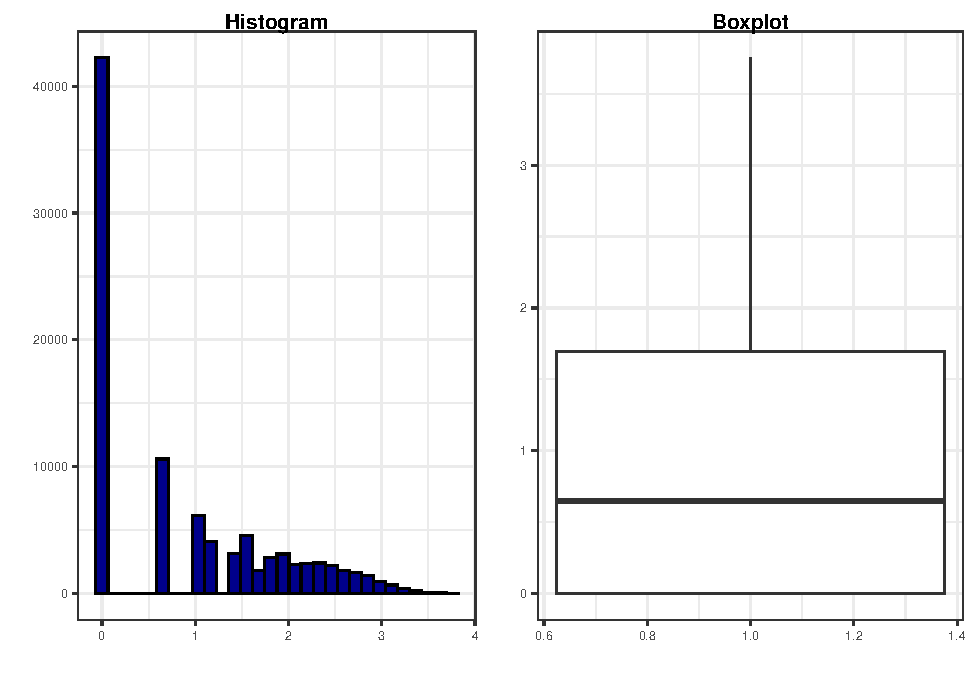
\includegraphics{_main_files/figure-latex/unnamed-chunk-51-1.pdf}

\hypertarget{unique-product-qty}{%
\subsection{Unique product qty}\label{unique-product-qty}}

\begin{Shaded}
\begin{Highlighting}[]
\FunctionTok{grid.draw}\NormalTok{(eda\_unbalanced}\SpecialCharTok{$}\NormalTok{unique\_product\_qty)}
\end{Highlighting}
\end{Shaded}

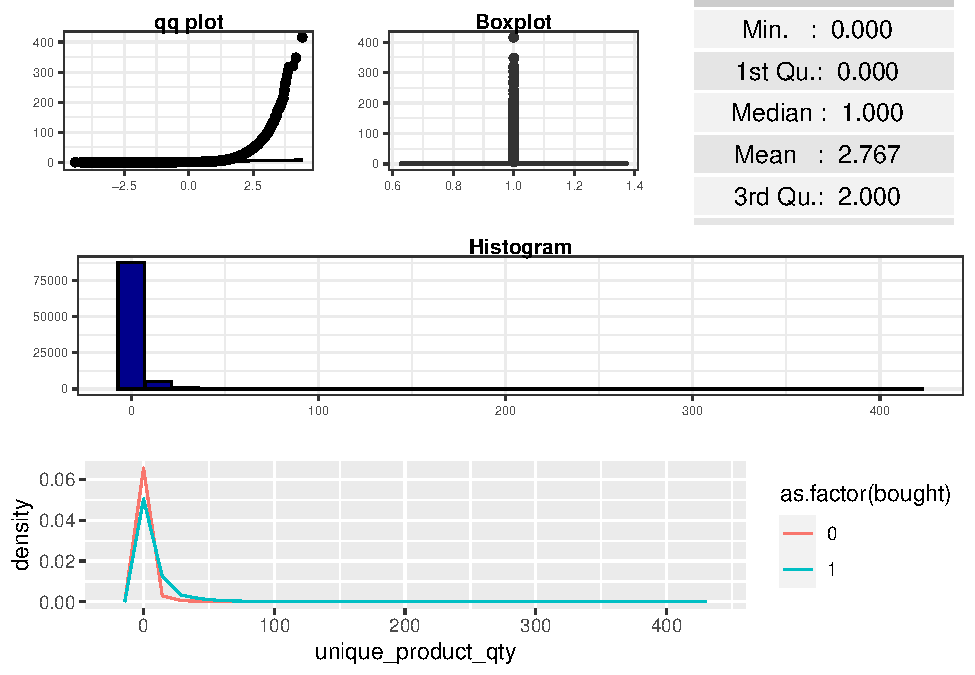
\includegraphics{_main_files/figure-latex/unnamed-chunk-52-1.pdf}

\begin{Shaded}
\begin{Highlighting}[]
\FunctionTok{grid.draw}\NormalTok{(eda\_balanced}\SpecialCharTok{$}\NormalTok{unique\_product\_qty)}
\end{Highlighting}
\end{Shaded}

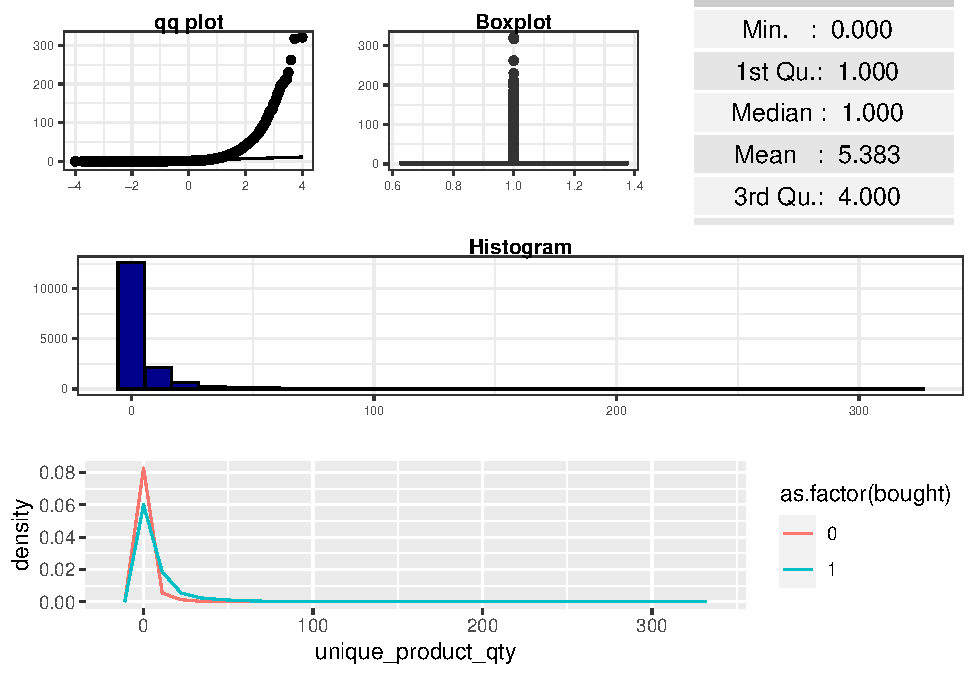
\includegraphics{_main_files/figure-latex/unnamed-chunk-53-1.pdf}

left skwed apply log transform

\begin{Shaded}
\begin{Highlighting}[]
\NormalTok{lambda }\OtherTok{\textless{}{-}} \FunctionTok{BoxCox.lambda}\NormalTok{(unbalanced\_data}\SpecialCharTok{$}\NormalTok{unique\_product\_qty, }\AttributeTok{method =} \StringTok{"guerrero"}\NormalTok{)  }
\end{Highlighting}
\end{Shaded}

\begin{verbatim}
## Warning in guerrero(x, lower, upper): Guerrero's method for selecting a Box-Cox
## parameter (lambda) is given for strictly positive data.
\end{verbatim}

\begin{Shaded}
\begin{Highlighting}[]
\NormalTok{histogram\_log }\OtherTok{\textless{}{-}} \FunctionTok{ggplot}\NormalTok{(unbalanced\_data, }\FunctionTok{aes}\NormalTok{(}\AttributeTok{x =} \FunctionTok{log}\NormalTok{(unique\_product\_qty))) }\SpecialCharTok{+}
    \FunctionTok{geom\_histogram}\NormalTok{(}\AttributeTok{fill=}\StringTok{"darkblue"}\NormalTok{, }\AttributeTok{color=}\StringTok{"black"}\NormalTok{) }\SpecialCharTok{+}
    \FunctionTok{theme\_masterDS}\NormalTok{() }\SpecialCharTok{+}
    \FunctionTok{labs}\NormalTok{(}
      \AttributeTok{x =} \StringTok{""}\NormalTok{,}
      \AttributeTok{y =} \StringTok{""}\NormalTok{,}
      \AttributeTok{title =} \StringTok{"Histogram"}
\NormalTok{    )}
  
\NormalTok{  boxplot\_log }\OtherTok{\textless{}{-}} \FunctionTok{ggplot}\NormalTok{(unbalanced\_data, }\FunctionTok{aes}\NormalTok{(}\AttributeTok{x =} \DecValTok{1}\NormalTok{, }\AttributeTok{y =} \FunctionTok{log}\NormalTok{(unique\_product\_qty))) }\SpecialCharTok{+}
    \FunctionTok{geom\_boxplot}\NormalTok{() }\SpecialCharTok{+}
    \FunctionTok{theme\_masterDS}\NormalTok{()}\SpecialCharTok{+}
    \FunctionTok{labs}\NormalTok{(}
      \AttributeTok{x =} \StringTok{""}\NormalTok{,}
      \AttributeTok{y=}\StringTok{""}\NormalTok{,}
      \AttributeTok{title =} \StringTok{"Boxplot"}
\NormalTok{    )}

  \FunctionTok{grid.arrange}\NormalTok{(histogram\_log, boxplot\_log, }\AttributeTok{nrow =} \DecValTok{1}\NormalTok{)}
\end{Highlighting}
\end{Shaded}

\begin{verbatim}
## `stat_bin()` using `bins = 30`. Pick better value with `binwidth`.
\end{verbatim}

\begin{verbatim}
## Warning: Removed 28829 rows containing non-finite values (stat_bin).
\end{verbatim}

\begin{verbatim}
## Warning: Removed 28829 rows containing non-finite values (stat_boxplot).
\end{verbatim}

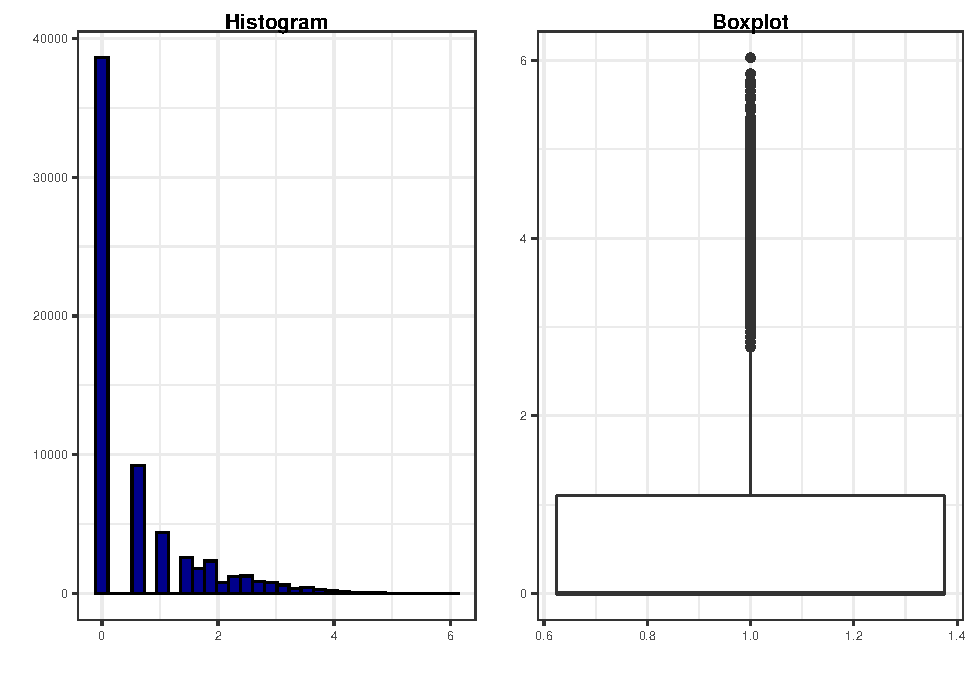
\includegraphics{_main_files/figure-latex/unnamed-chunk-54-1.pdf}

\hypertarget{unique-browse-designer-quantity}{%
\subsection{Unique browse designer quantity}\label{unique-browse-designer-quantity}}

\begin{Shaded}
\begin{Highlighting}[]
\FunctionTok{grid.draw}\NormalTok{(eda\_unbalanced}\SpecialCharTok{$}\NormalTok{unique\_browse\_designer\_qty)}
\end{Highlighting}
\end{Shaded}

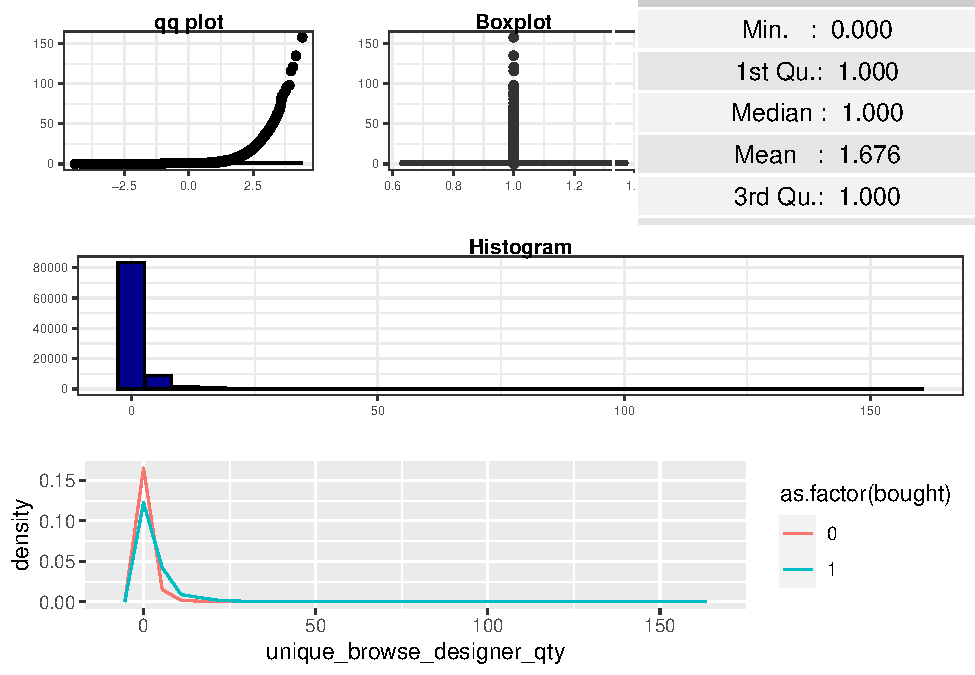
\includegraphics{_main_files/figure-latex/unnamed-chunk-55-1.pdf}

\begin{Shaded}
\begin{Highlighting}[]
\FunctionTok{grid.draw}\NormalTok{(eda\_balanced}\SpecialCharTok{$}\NormalTok{unique\_browse\_designer\_qty)}
\end{Highlighting}
\end{Shaded}

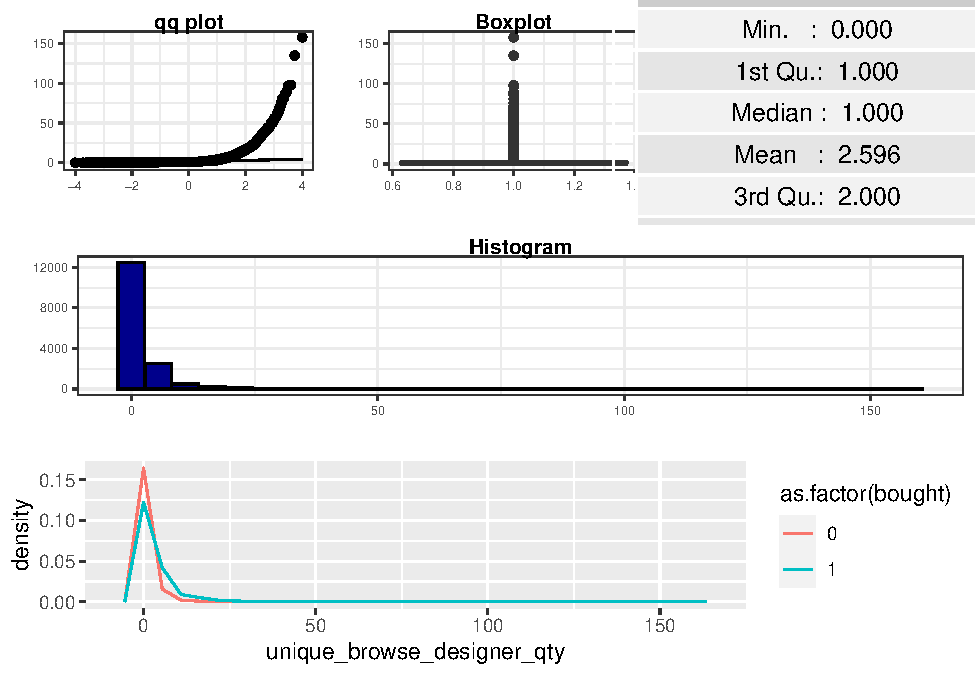
\includegraphics{_main_files/figure-latex/unnamed-chunk-56-1.pdf}

left skwed apply log transform

\begin{Shaded}
\begin{Highlighting}[]
\NormalTok{ histogram\_log }\OtherTok{\textless{}{-}} \FunctionTok{ggplot}\NormalTok{(unbalanced\_data, }\FunctionTok{aes}\NormalTok{(}\AttributeTok{x =} \FunctionTok{log}\NormalTok{(unique\_browse\_designer\_qty))) }\SpecialCharTok{+}
    \FunctionTok{geom\_histogram}\NormalTok{(}\AttributeTok{fill=}\StringTok{"darkblue"}\NormalTok{, }\AttributeTok{color=}\StringTok{"black"}\NormalTok{) }\SpecialCharTok{+}
    \FunctionTok{theme\_masterDS}\NormalTok{() }\SpecialCharTok{+}
    \FunctionTok{labs}\NormalTok{(}
      \AttributeTok{x =} \StringTok{""}\NormalTok{,}
      \AttributeTok{y =} \StringTok{""}\NormalTok{,}
      \AttributeTok{title =} \StringTok{"Histogram"}
\NormalTok{    )}
  
\NormalTok{  boxplot\_log }\OtherTok{\textless{}{-}} \FunctionTok{ggplot}\NormalTok{(unbalanced\_data, }\FunctionTok{aes}\NormalTok{(}\AttributeTok{x =} \DecValTok{1}\NormalTok{, }\AttributeTok{y =} \FunctionTok{log}\NormalTok{(unique\_browse\_designer\_qty))) }\SpecialCharTok{+}
    \FunctionTok{geom\_boxplot}\NormalTok{() }\SpecialCharTok{+}
    \FunctionTok{theme\_masterDS}\NormalTok{()}\SpecialCharTok{+}
    \FunctionTok{labs}\NormalTok{(}
      \AttributeTok{x =} \StringTok{""}\NormalTok{,}
      \AttributeTok{y=}\StringTok{""}\NormalTok{,}
      \AttributeTok{title =} \StringTok{"Boxplot"}
\NormalTok{    )}

  \FunctionTok{grid.arrange}\NormalTok{(histogram\_log, boxplot\_log, }\AttributeTok{nrow =} \DecValTok{1}\NormalTok{)}
\end{Highlighting}
\end{Shaded}

\begin{verbatim}
## `stat_bin()` using `bins = 30`. Pick better value with `binwidth`.
\end{verbatim}

\begin{verbatim}
## Warning: Removed 14778 rows containing non-finite values (stat_bin).
\end{verbatim}

\begin{verbatim}
## Warning: Removed 14778 rows containing non-finite values (stat_boxplot).
\end{verbatim}

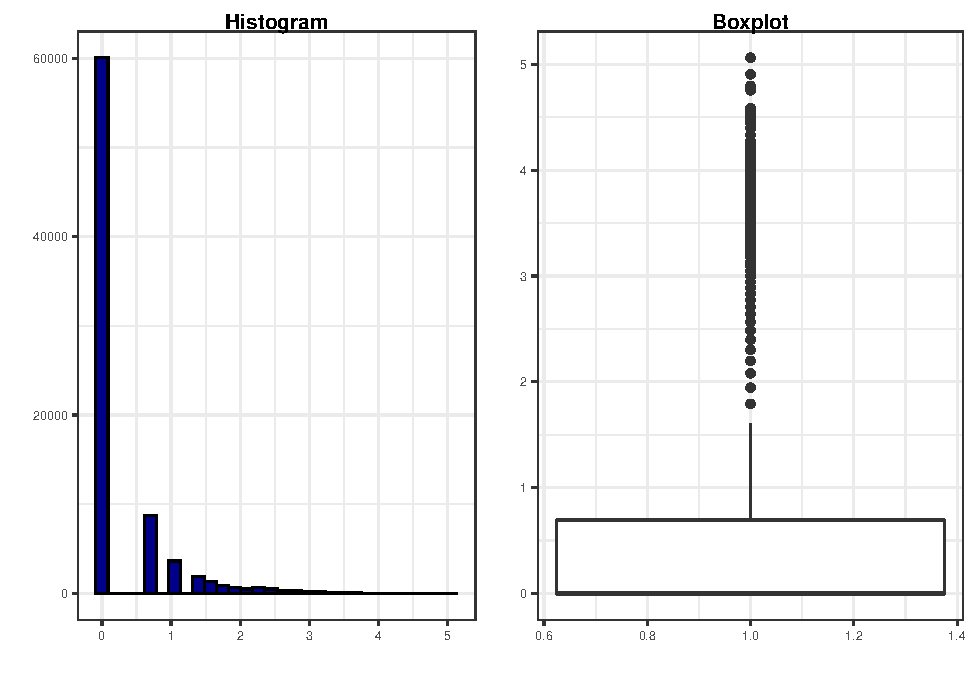
\includegraphics{_main_files/figure-latex/unnamed-chunk-57-1.pdf}

\begin{Shaded}
\begin{Highlighting}[]
\NormalTok{ histogram\_log }\OtherTok{\textless{}{-}} \FunctionTok{ggplot}\NormalTok{(unbalanced\_data, }\FunctionTok{aes}\NormalTok{(}\AttributeTok{x =}\NormalTok{ unique\_browse\_designer\_qty}\SpecialCharTok{/}\NormalTok{view\_qty)) }\SpecialCharTok{+}
    \FunctionTok{geom\_histogram}\NormalTok{(}\AttributeTok{fill=}\StringTok{"darkblue"}\NormalTok{, }\AttributeTok{color=}\StringTok{"black"}\NormalTok{) }\SpecialCharTok{+}
    \FunctionTok{theme\_masterDS}\NormalTok{() }\SpecialCharTok{+}
    \FunctionTok{labs}\NormalTok{(}
      \AttributeTok{x =} \StringTok{""}\NormalTok{,}
      \AttributeTok{y =} \StringTok{""}\NormalTok{,}
      \AttributeTok{title =} \StringTok{"Histogram"}
\NormalTok{    )}
  
\NormalTok{  boxplot\_log }\OtherTok{\textless{}{-}} \FunctionTok{ggplot}\NormalTok{(unbalanced\_data, }\FunctionTok{aes}\NormalTok{(}\AttributeTok{x =} \DecValTok{1}\NormalTok{, }\AttributeTok{y =}\NormalTok{ unique\_browse\_designer\_qty}\SpecialCharTok{/}\NormalTok{view\_qty)) }\SpecialCharTok{+}
    \FunctionTok{geom\_boxplot}\NormalTok{() }\SpecialCharTok{+}
    \FunctionTok{theme\_masterDS}\NormalTok{()}\SpecialCharTok{+}
    \FunctionTok{labs}\NormalTok{(}
      \AttributeTok{x =} \StringTok{""}\NormalTok{,}
      \AttributeTok{y=}\StringTok{""}\NormalTok{,}
      \AttributeTok{title =} \StringTok{"Boxplot"}
\NormalTok{    )}

  \FunctionTok{grid.arrange}\NormalTok{(histogram\_log, boxplot\_log, }\AttributeTok{nrow =} \DecValTok{1}\NormalTok{)}
\end{Highlighting}
\end{Shaded}

\begin{verbatim}
## `stat_bin()` using `bins = 30`. Pick better value with `binwidth`.
\end{verbatim}

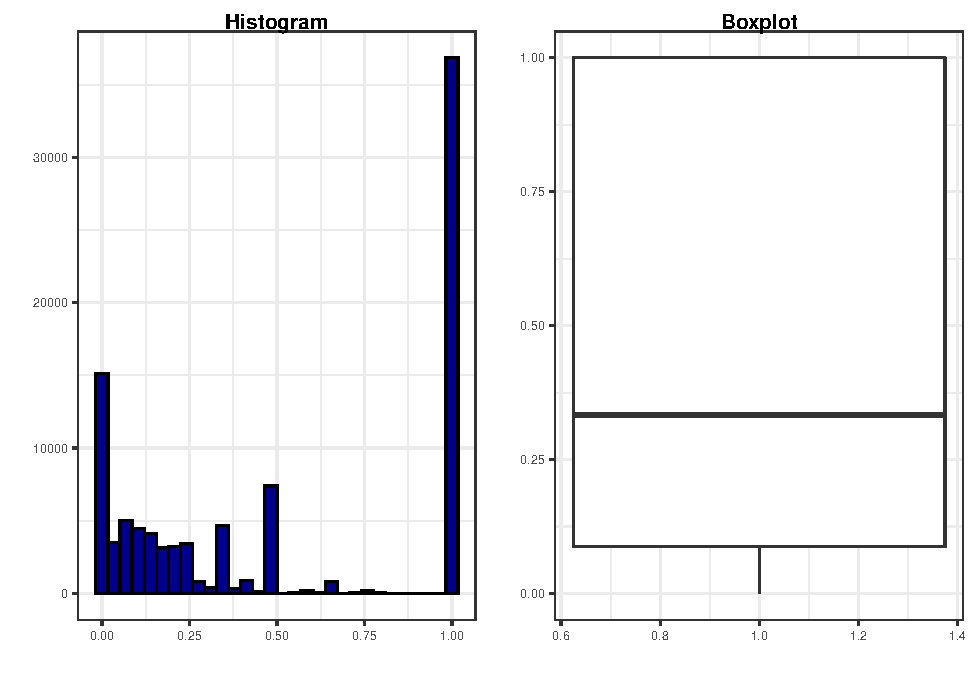
\includegraphics{_main_files/figure-latex/unnamed-chunk-58-1.pdf}

\hypertarget{is-subscribed}{%
\subsection{Is subscribed}\label{is-subscribed}}

\begin{Shaded}
\begin{Highlighting}[]
\FunctionTok{grid.draw}\NormalTok{(eda\_unbalanced}\SpecialCharTok{$}\NormalTok{is\_subscribed)}
\end{Highlighting}
\end{Shaded}

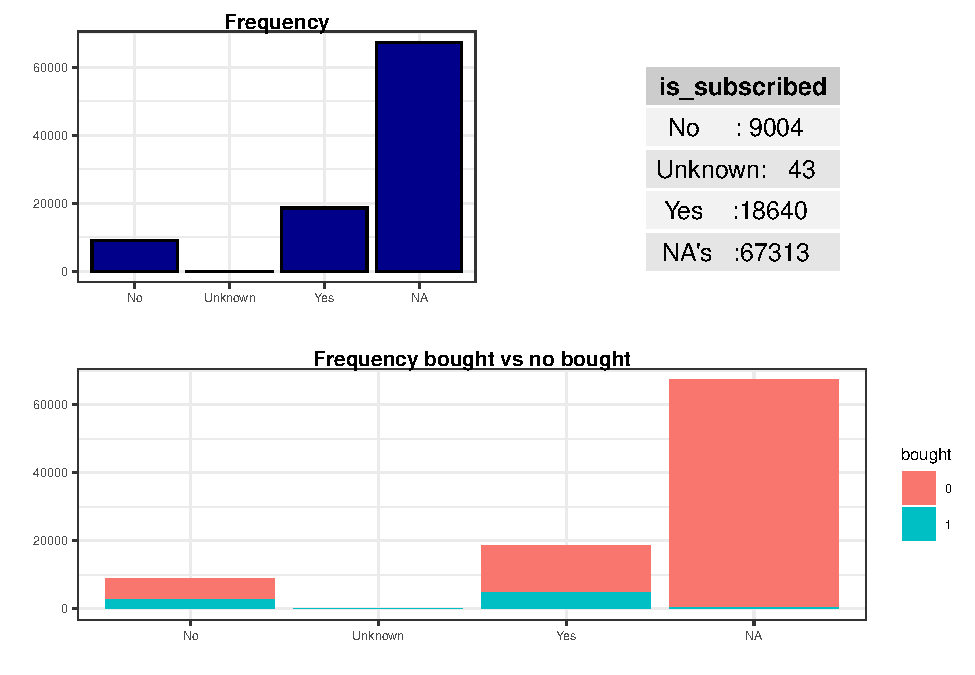
\includegraphics{_main_files/figure-latex/unnamed-chunk-59-1.pdf}

\begin{Shaded}
\begin{Highlighting}[]
\FunctionTok{grid.draw}\NormalTok{(eda\_balanced}\SpecialCharTok{$}\NormalTok{is\_subscribed)}
\end{Highlighting}
\end{Shaded}

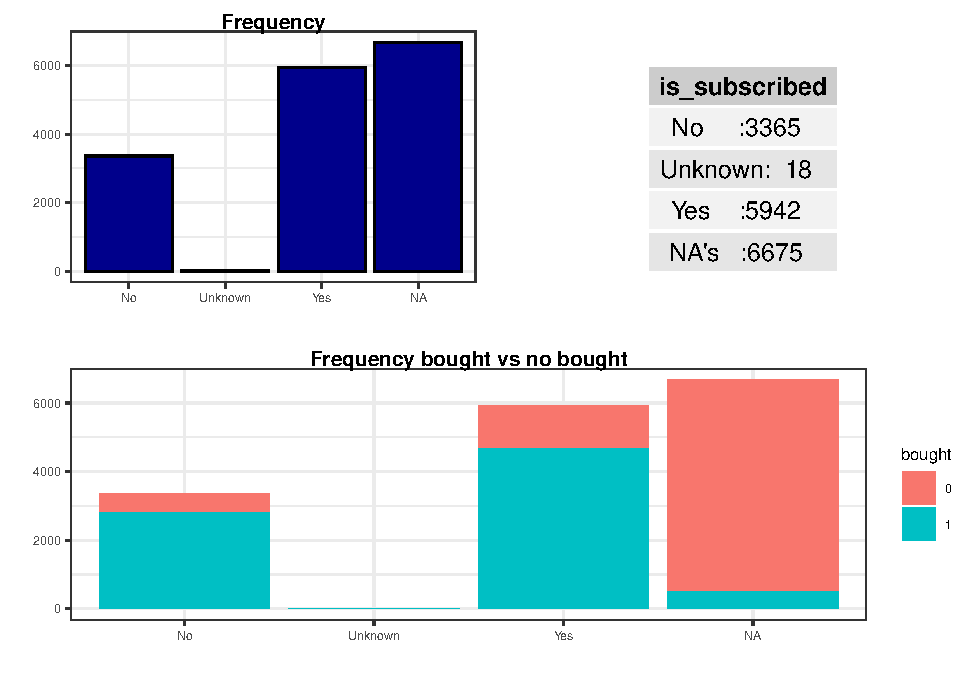
\includegraphics{_main_files/figure-latex/unnamed-chunk-60-1.pdf}

For both datasets the class majority is NA. From the information given we cannot conclude that we can remove this feature from the model, and given the number of observations affected we will look for imputation alternatives.

If a particular variable is having more missing values that rest of the variables in the dataset, and, if by removing that one variable you can save many observations. I would, then, suggest to remove that particular variable, unless it is a really important predictor that makes a lot of business sense. It is a matter of deciding between the importance of the variable and losing out on a number of observation.

Given that its a categorical variable we could replace with the mode, and that would mean that all NA would become Yes, but given the size of missing values this can return a huge impact. We will explore statitical imputation using knn.

DMwR::knnImputation uses k-Nearest Neighbours approach to impute missing values. What kNN imputation does in simpler terms is as follows: For every observation to be imputed, it identifies `k' closest observations based on the euclidean distance and computes the weighted average (weighted based on distance) of these `k' obs.

\hypertarget{browser-name}{%
\subsection{Browser name}\label{browser-name}}

\begin{Shaded}
\begin{Highlighting}[]
\FunctionTok{grid.draw}\NormalTok{(eda\_unbalanced}\SpecialCharTok{$}\NormalTok{browser\_name)}
\end{Highlighting}
\end{Shaded}

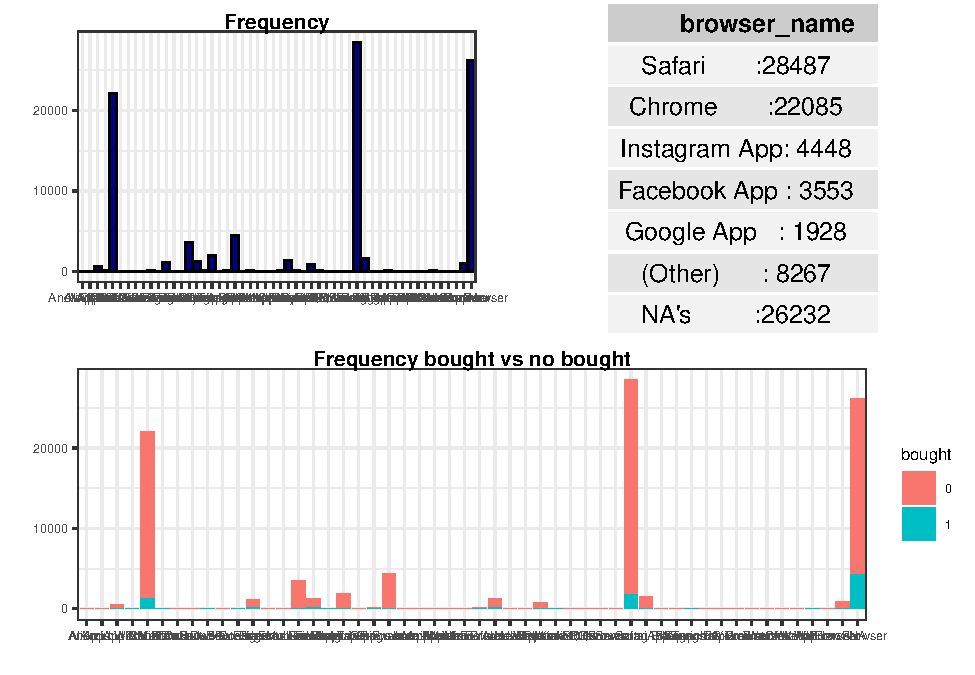
\includegraphics{_main_files/figure-latex/unnamed-chunk-61-1.pdf}

\begin{Shaded}
\begin{Highlighting}[]
\FunctionTok{grid.draw}\NormalTok{(eda\_balanced}\SpecialCharTok{$}\NormalTok{browser\_name)}
\end{Highlighting}
\end{Shaded}

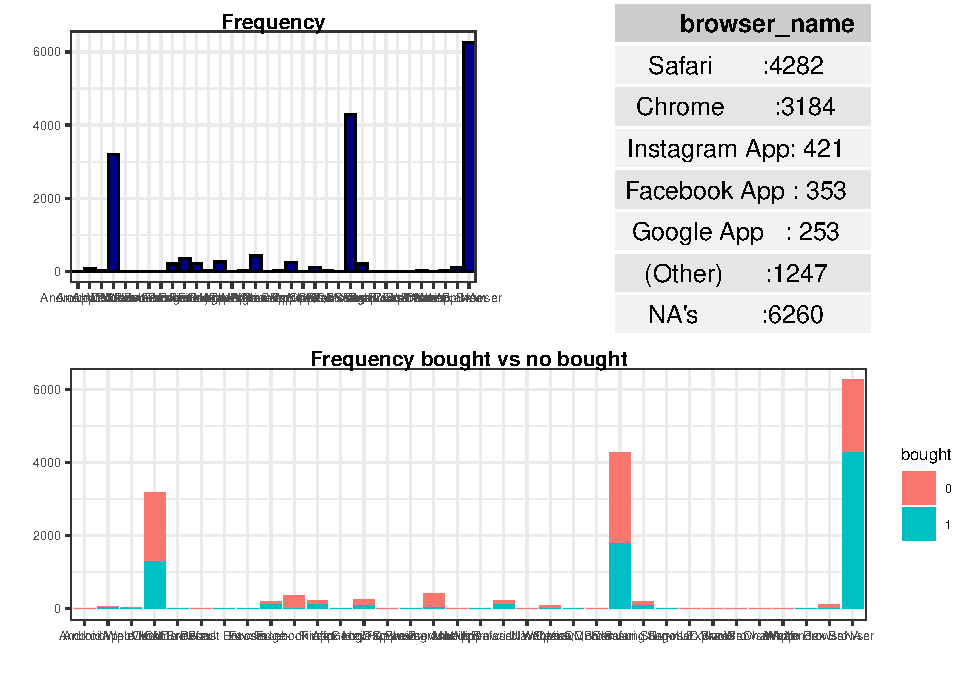
\includegraphics{_main_files/figure-latex/unnamed-chunk-62-1.pdf}

\hypertarget{country}{%
\subsection{Country}\label{country}}

\begin{Shaded}
\begin{Highlighting}[]
\FunctionTok{grid.draw}\NormalTok{(eda\_unbalanced}\SpecialCharTok{$}\NormalTok{country)}
\end{Highlighting}
\end{Shaded}

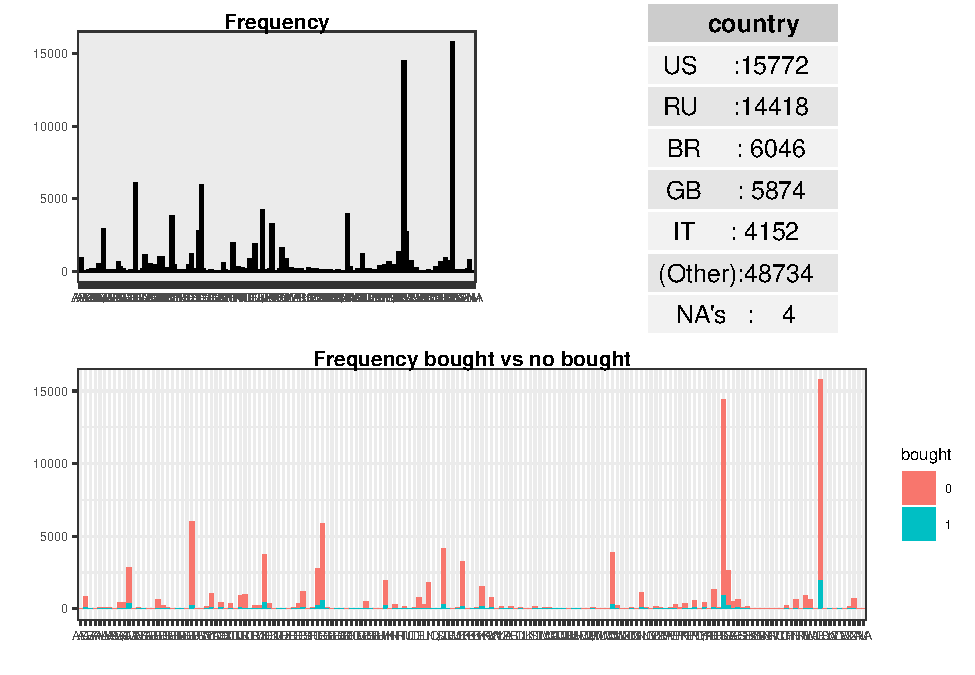
\includegraphics{_main_files/figure-latex/unnamed-chunk-63-1.pdf}

\begin{Shaded}
\begin{Highlighting}[]
\FunctionTok{grid.draw}\NormalTok{(eda\_balanced}\SpecialCharTok{$}\NormalTok{country)}
\end{Highlighting}
\end{Shaded}

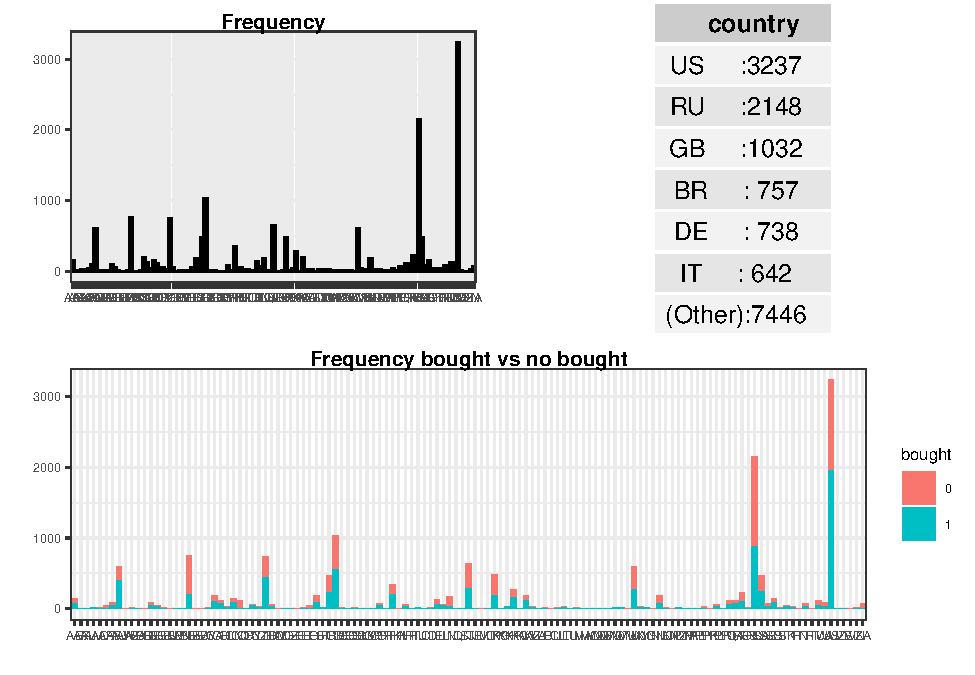
\includegraphics{_main_files/figure-latex/unnamed-chunk-64-1.pdf}

remove rows withna

\begin{Shaded}
\begin{Highlighting}[]
\NormalTok{correct\_data }\OtherTok{\textless{}{-}} \FunctionTok{select}\NormalTok{(unbalanced\_data, }\SpecialCharTok{{-}}\NormalTok{session\_id)}
\FunctionTok{summary}\NormalTok{(correct\_data)}
\end{Highlighting}
\end{Shaded}

\begin{verbatim}
##        plaform                         segment       customer_type  
##  mobile_app:26232   FFACCESS-Bronze        : 9331   customer:19471  
##  website   :68768   FFACCESS-Gold          : 2405   prospect:75529  
##                     FFACCESS-Platinum      : 1240                   
##                     FFACCESS-Private-Client: 1564                   
##                     FFACCESS-Silver        : 2511                   
##                     without_segment        :77949                   
##                                                                     
##      device_group      visitor_type   has_listing has_used_search
##  App       :26232   new      :48592   0:44979     0:80466        
##  Desktop   :16201   returning:46408   1:50021     1:14534        
##  Mobile Web:52567                                                
##                                                                  
##                                                                  
##                                                                  
##                                                                  
##  has_recommendation has_add_to_wishlist has_add_to_bag    duration      
##  0:65594            0:90468             0:84191        Min.   :    0.0  
##  1:29406            1: 4532             1:10809        1st Qu.:    0.0  
##                                                        Median :   15.0  
##                                                        Mean   :  332.5  
##                                                        3rd Qu.:  223.0  
##                                                        Max.   :20295.0  
##                                                                         
##     view_qty       unique_product_qty unique_browse_designer_qty
##  Min.   :   1.00   Min.   :  0.000    Min.   :  0.000           
##  1st Qu.:   1.00   1st Qu.:  0.000    1st Qu.:  1.000           
##  Median :   2.00   Median :  1.000    Median :  1.000           
##  Mean   :  10.97   Mean   :  2.767    Mean   :  1.676           
##  3rd Qu.:   8.00   3rd Qu.:  2.000    3rd Qu.:  1.000           
##  Max.   :1151.00   Max.   :416.000    Max.   :158.000           
##                                                                 
##  unique_browse_category_qty is_subscribed          browser_name  
##  1      :53094              No     : 9004   Safari       :28487  
##  0      :22498              Unknown:   43   Chrome       :22085  
##  2      :11476              Yes    :18640   Instagram App: 4448  
##  3      : 3834              NA's   :67313   Facebook App : 3553  
##  4      : 1795                              Google App   : 1928  
##  5      :  929                              (Other)      : 8267  
##  (Other): 1374                              NA's         :26232  
##     country      bought   
##  US     :15772   0:87000  
##  RU     :14418   1: 8000  
##  BR     : 6046            
##  GB     : 5874            
##  IT     : 4152            
##  (Other):48734            
##  NA's   :    4
\end{verbatim}

\begin{Shaded}
\begin{Highlighting}[]
\NormalTok{rec }\OtherTok{\textless{}{-}} \FunctionTok{recipe}\NormalTok{(bought }\SpecialCharTok{\textasciitilde{}}\NormalTok{ ., }\AttributeTok{data =}\NormalTok{ correct\_data)}

\NormalTok{ratio\_recipe }\OtherTok{\textless{}{-}}\NormalTok{ rec }\SpecialCharTok{\%\textgreater{}\%} 
  \FunctionTok{step\_impute\_knn}\NormalTok{(}\FunctionTok{all\_predictors}\NormalTok{(), }\AttributeTok{neighbors =} \DecValTok{3}\NormalTok{)}
\NormalTok{ratio\_recipe2 }\OtherTok{\textless{}{-}} \FunctionTok{prep}\NormalTok{(ratio\_recipe, }\AttributeTok{training =}\NormalTok{ unbalanced\_data, }\AttributeTok{verbose =} \ConstantTok{TRUE}\NormalTok{, }\AttributeTok{retain =} \ConstantTok{TRUE}\NormalTok{)}
\end{Highlighting}
\end{Shaded}

\begin{verbatim}
## oper 1 step impute knn [training] 
## The retained training set is ~ 8.36 Mb  in memory.
\end{verbatim}

\begin{Shaded}
\begin{Highlighting}[]
\NormalTok{imputed }\OtherTok{\textless{}{-}} \FunctionTok{bake}\NormalTok{(ratio\_recipe2,}\AttributeTok{new\_data =} \ConstantTok{NULL}\NormalTok{)}
\FunctionTok{summary}\NormalTok{(imputed)}
\end{Highlighting}
\end{Shaded}

\begin{verbatim}
##        plaform                         segment       customer_type  
##  mobile_app:26232   FFACCESS-Bronze        : 9331   customer:19471  
##  website   :68768   FFACCESS-Gold          : 2405   prospect:75529  
##                     FFACCESS-Platinum      : 1240                   
##                     FFACCESS-Private-Client: 1564                   
##                     FFACCESS-Silver        : 2511                   
##                     without_segment        :77949                   
##                                                                     
##      device_group      visitor_type   has_listing has_used_search
##  App       :26232   new      :48592   0:44979     0:80466        
##  Desktop   :16201   returning:46408   1:50021     1:14534        
##  Mobile Web:52567                                                
##                                                                  
##                                                                  
##                                                                  
##                                                                  
##  has_recommendation has_add_to_wishlist has_add_to_bag    duration      
##  0:65594            0:90468             0:84191        Min.   :    0.0  
##  1:29406            1: 4532             1:10809        1st Qu.:    0.0  
##                                                        Median :   15.0  
##                                                        Mean   :  332.5  
##                                                        3rd Qu.:  223.0  
##                                                        Max.   :20295.0  
##                                                                         
##     view_qty       unique_product_qty unique_browse_designer_qty
##  Min.   :   1.00   Min.   :  0.000    Min.   :  0.000           
##  1st Qu.:   1.00   1st Qu.:  0.000    1st Qu.:  1.000           
##  Median :   2.00   Median :  1.000    Median :  1.000           
##  Mean   :  10.97   Mean   :  2.767    Mean   :  1.676           
##  3rd Qu.:   8.00   3rd Qu.:  2.000    3rd Qu.:  1.000           
##  Max.   :1151.00   Max.   :416.000    Max.   :158.000           
##                                                                 
##  unique_browse_category_qty is_subscribed            browser_name  
##  1      :53094              No     :39612   Safari         :39038  
##  0      :22498              Unknown:   44   Chrome         :33345  
##  2      :11476              Yes    :55344   Instagram App  : 5076  
##  3      : 3834                              Facebook App   : 3779  
##  4      : 1795                              Google App     : 2567  
##  5      :  929                              Samsung Browser: 2182  
##  (Other): 1374                              (Other)        : 9013  
##     country      bought   
##  US     :15772   0:87000  
##  RU     :14419   1: 8000  
##  BR     : 6046            
##  GB     : 5874            
##  IT     : 4152            
##  MX     : 3903            
##  (Other):44834
\end{verbatim}

\hypertarget{assess-data-quality-transformations-to-be-made}{%
\section{Assess data quality \& transformations to be made}\label{assess-data-quality-transformations-to-be-made}}

\begin{Shaded}
\begin{Highlighting}[]
\FunctionTok{md.pattern}\NormalTok{(unbalanced\_data, }\AttributeTok{rotate.names =} \ConstantTok{TRUE}\NormalTok{)}
\end{Highlighting}
\end{Shaded}

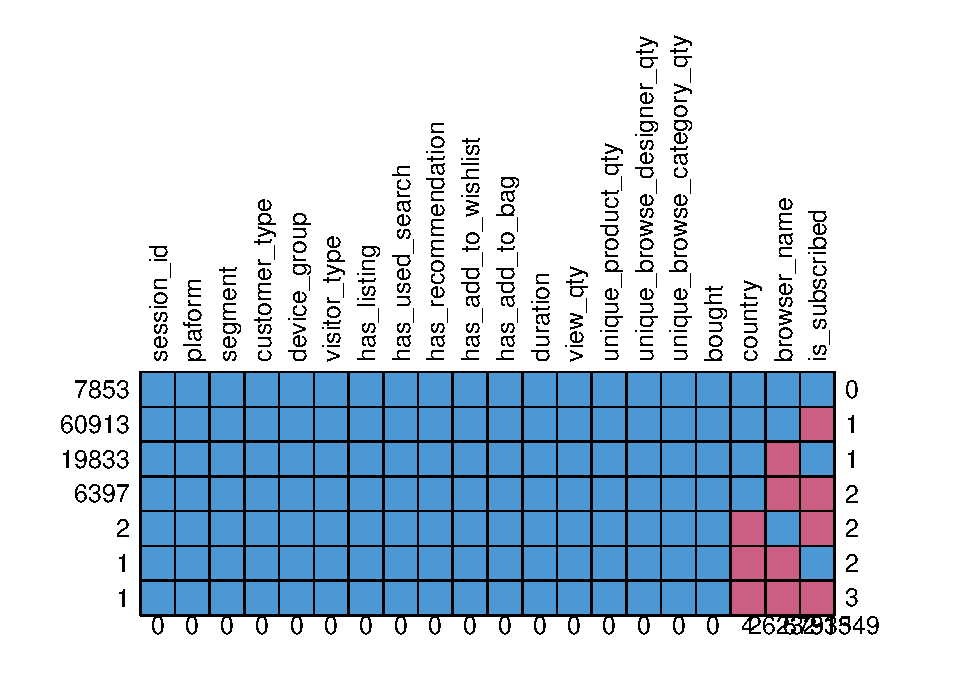
\includegraphics{_main_files/figure-latex/unnamed-chunk-66-1.pdf}

\begin{verbatim}
##       session_id plaform segment customer_type device_group visitor_type
## 7853           1       1       1             1            1            1
## 60913          1       1       1             1            1            1
## 19833          1       1       1             1            1            1
## 6397           1       1       1             1            1            1
## 2              1       1       1             1            1            1
## 1              1       1       1             1            1            1
## 1              1       1       1             1            1            1
##                0       0       0             0            0            0
##       has_listing has_used_search has_recommendation has_add_to_wishlist
## 7853            1               1                  1                   1
## 60913           1               1                  1                   1
## 19833           1               1                  1                   1
## 6397            1               1                  1                   1
## 2               1               1                  1                   1
## 1               1               1                  1                   1
## 1               1               1                  1                   1
##                 0               0                  0                   0
##       has_add_to_bag duration view_qty unique_product_qty
## 7853               1        1        1                  1
## 60913              1        1        1                  1
## 19833              1        1        1                  1
## 6397               1        1        1                  1
## 2                  1        1        1                  1
## 1                  1        1        1                  1
## 1                  1        1        1                  1
##                    0        0        0                  0
##       unique_browse_designer_qty unique_browse_category_qty bought country
## 7853                           1                          1      1       1
## 60913                          1                          1      1       1
## 19833                          1                          1      1       1
## 6397                           1                          1      1       1
## 2                              1                          1      1       0
## 1                              1                          1      1       0
## 1                              1                          1      1       0
##                                0                          0      0       4
##       browser_name is_subscribed      
## 7853             1             1     0
## 60913            1             0     1
## 19833            0             1     1
## 6397             0             0     2
## 2                1             0     2
## 1                0             1     2
## 1                0             0     3
##              26232         67313 93549
\end{verbatim}

\begin{Shaded}
\begin{Highlighting}[]
\FunctionTok{md.pattern}\NormalTok{(balanced\_data,}\AttributeTok{rotate.names =} \ConstantTok{TRUE}\NormalTok{)}
\end{Highlighting}
\end{Shaded}

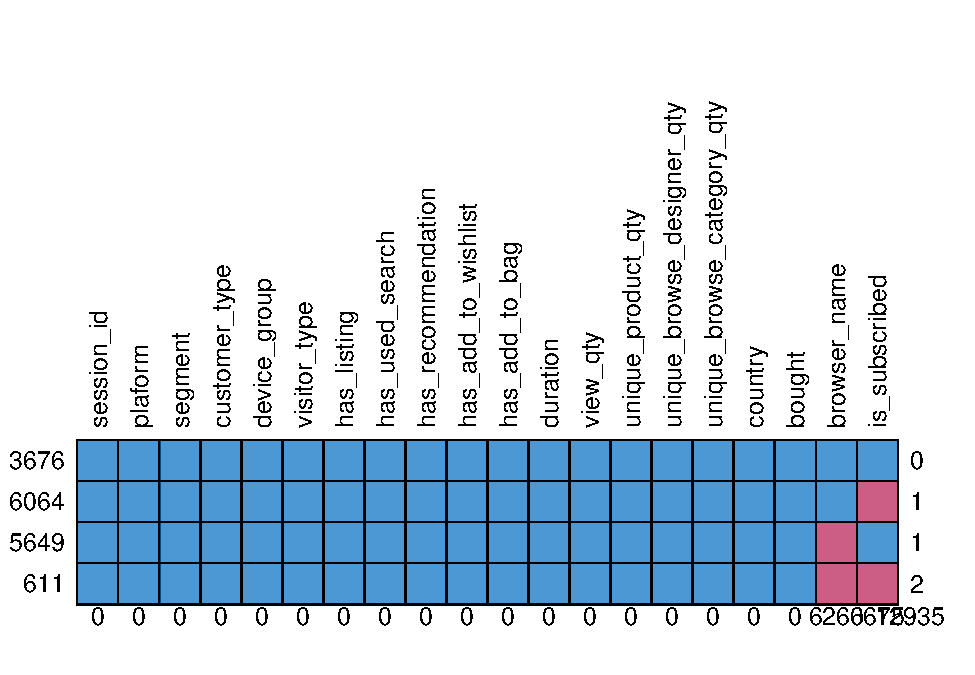
\includegraphics{_main_files/figure-latex/unnamed-chunk-67-1.pdf}

\begin{verbatim}
##      session_id plaform segment customer_type device_group visitor_type
## 3676          1       1       1             1            1            1
## 6064          1       1       1             1            1            1
## 5649          1       1       1             1            1            1
## 611           1       1       1             1            1            1
##               0       0       0             0            0            0
##      has_listing has_used_search has_recommendation has_add_to_wishlist
## 3676           1               1                  1                   1
## 6064           1               1                  1                   1
## 5649           1               1                  1                   1
## 611            1               1                  1                   1
##                0               0                  0                   0
##      has_add_to_bag duration view_qty unique_product_qty
## 3676              1        1        1                  1
## 6064              1        1        1                  1
## 5649              1        1        1                  1
## 611               1        1        1                  1
##                   0        0        0                  0
##      unique_browse_designer_qty unique_browse_category_qty country bought
## 3676                          1                          1       1      1
## 6064                          1                          1       1      1
## 5649                          1                          1       1      1
## 611                           1                          1       1      1
##                               0                          0       0      0
##      browser_name is_subscribed      
## 3676            1             1     0
## 6064            1             0     1
## 5649            0             1     1
## 611             0             0     2
##              6260          6675 12935
\end{verbatim}

\hypertarget{summary-of-findings}{%
\section{Summary of findings}\label{summary-of-findings}}

\begin{itemize}
\tightlist
\item
  Device group and platform have a strong relationship and should be taken into consideration during transformations.
\item
  Features conserning journey can have strong intereactions between then which should be taken into consideration during the model
\item
  The graphical analysis already provides a important insight given the business objectives. From the unbalanced data available we can conclude that around of 46\% shopping carts are lost on that session. That raises a question of how are this recovered (example on a next session) or if this means that all this sales are lost right at the end of the sales funnel.
\item
  Log transform duration
\item
  Log transform view\_qty and remove below or after tukeys value
\item
  Log transform unique\_qty remove below or after tukeys value
\item
  Log transform nique browse designer quantity remove below or after tukeys value
\item
  remove rows with na country
\end{itemize}

  \bibliography{book.bib,packages.bib}

\end{document}
